%# -*- coding: utf-8-unix -*-
%%==================================================
%% thesis.tex
%%==================================================

% 双面打印
%\documentclass[doctor, fontset=adobe, openright, twoside]{sjtuthesis}
% \documentclass[bachelor, fontset=adobe, openany, oneside, submit]{sjtuthesis}
\documentclass[master, fontset=adobe, submit]{sjtuthesis}
% \documentclass[%
%   bachelor|master|doctor,	% 必选项
%   fontset=adobe|windows,  	% 只测试了adobe
%   oneside|twoside,		% 单面打印,双面打印(奇偶页交换页边距,默认)
%   openany|openright, 		% 可以在奇数或者偶数页开新章|只在奇数页开新章(默认)
%   zihao=-4|5,, 		% 正文字号:小四、五号(默认)
%   review,	 		% 盲审论文,隐去作者姓名、学号、导师姓名、致谢、发表论文和参与的项目
%   submit			% 定稿提交的论文,插入签名扫描版的原创性声明、授权声明 
% ]

% 逐个导入参考文献数据库
\addbibresource{bib/thesis.bib}
% \addbibresource{bib/chap2.bib}

\begin{document}

%% 无编号内容:中英文论文封面、授权页
%# -*- coding: utf-8-unix -*-
\title{基于Clearwater的网络功能虚拟化资源分配模型研究}
\author{李\quad{}阳德}
\advisor{李健\quad{}副教授}
% \coadvisor{某某教授}
\defenddate{2018年1月12日}
\school{上海交通大学}
\institute{软件学院}
\studentnumber{115037910070}
\major{软件工程}

\englishtitle{Research on Resource Allocation of Network Function Virtualization on Clearwater Platform}
\englishauthor{\textsc{Yangde Li}}
\englishadvisor{Prof. \textsc{Jian Li}}
% \englishcoadvisor{Prof. \textsc{Uom Uom}}
\englishschool{Shanghai Jiao Tong University}
\englishinstitute{\textsc{Depart of Software Engineering, School of Electronics and Electric Engineering} \\
  \textsc{Shanghai Jiao Tong University} \\
  \textsc{Shanghai, P.R.China}}
\englishmajor{Software Engineering}
\englishdate{Dec. 17th, 2018}


\maketitle

\makeenglishtitle

\makeatletter
\ifsjtu@submit\relax
	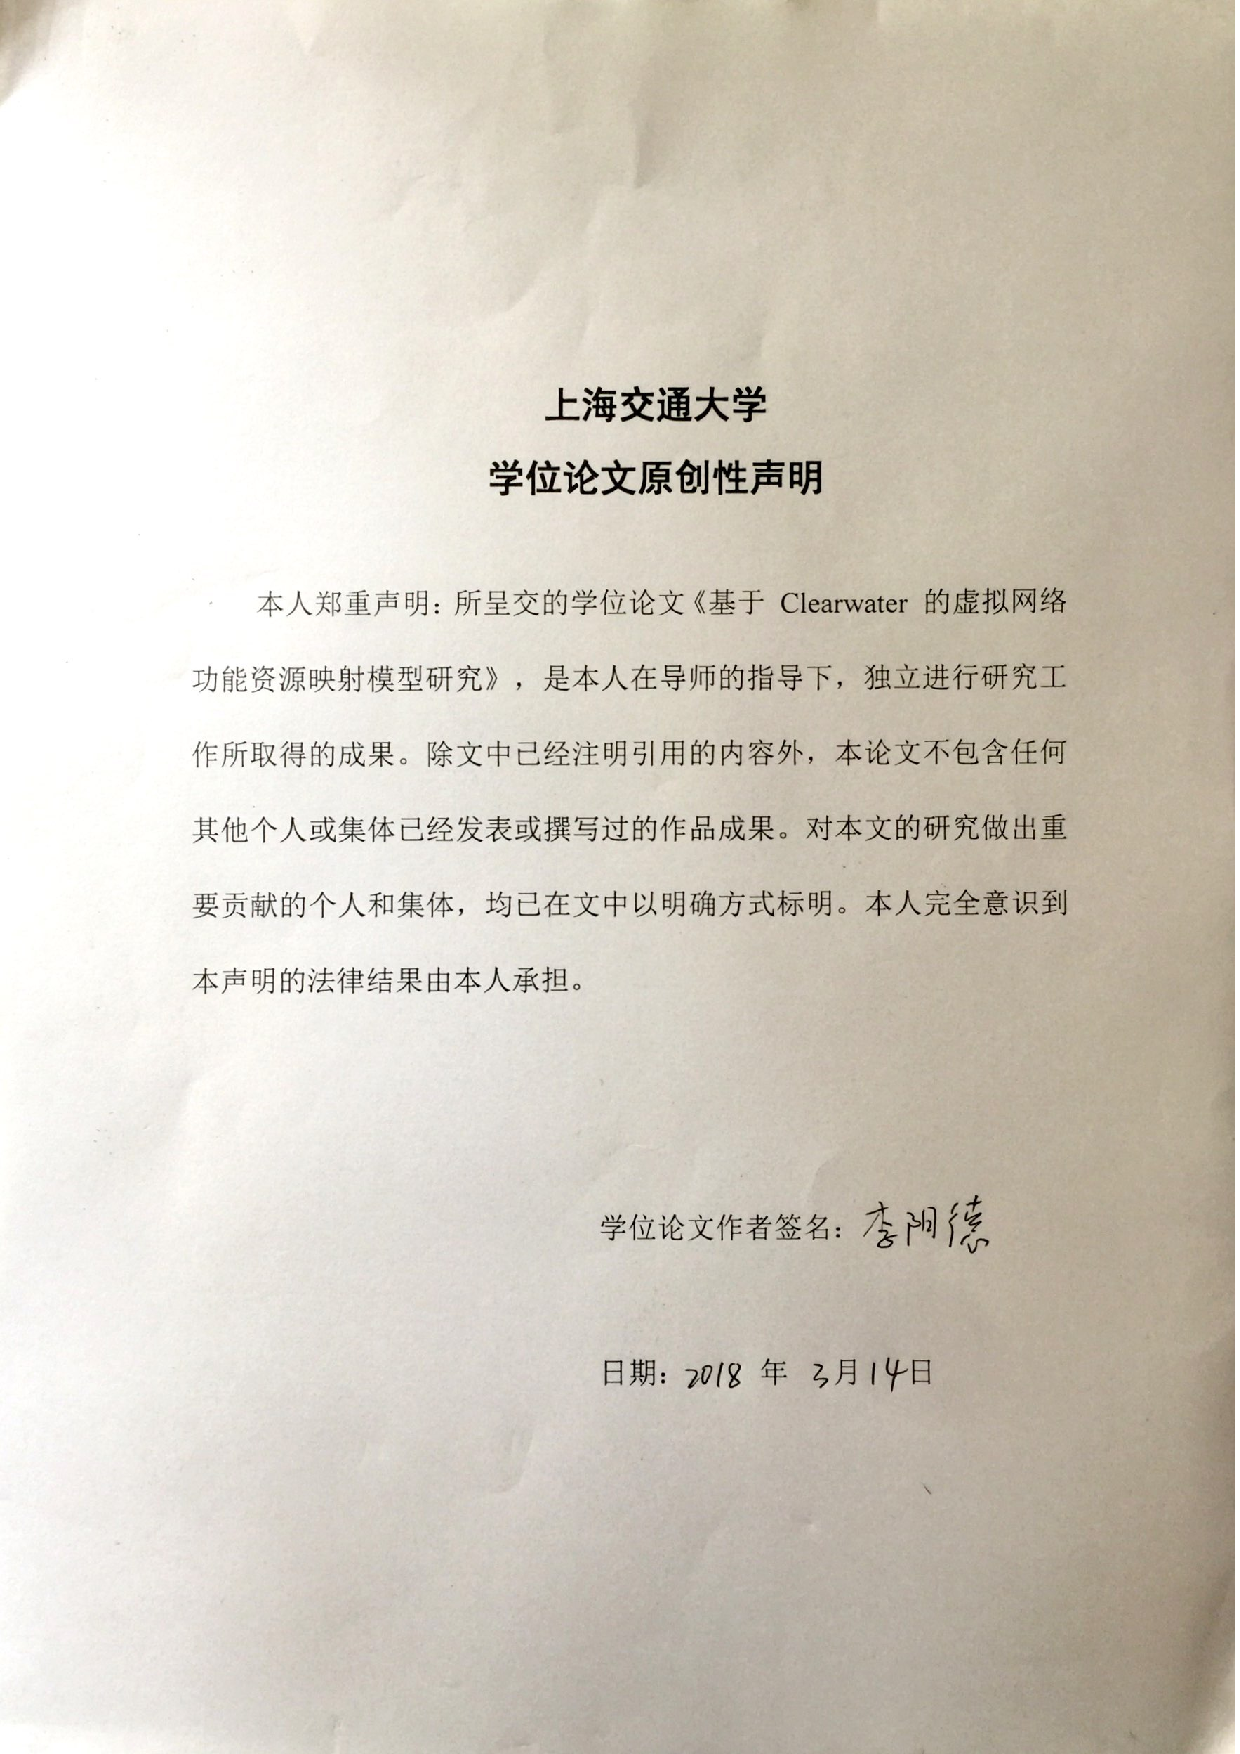
\includepdf{pdf/original.pdf}
	\cleardoublepage
	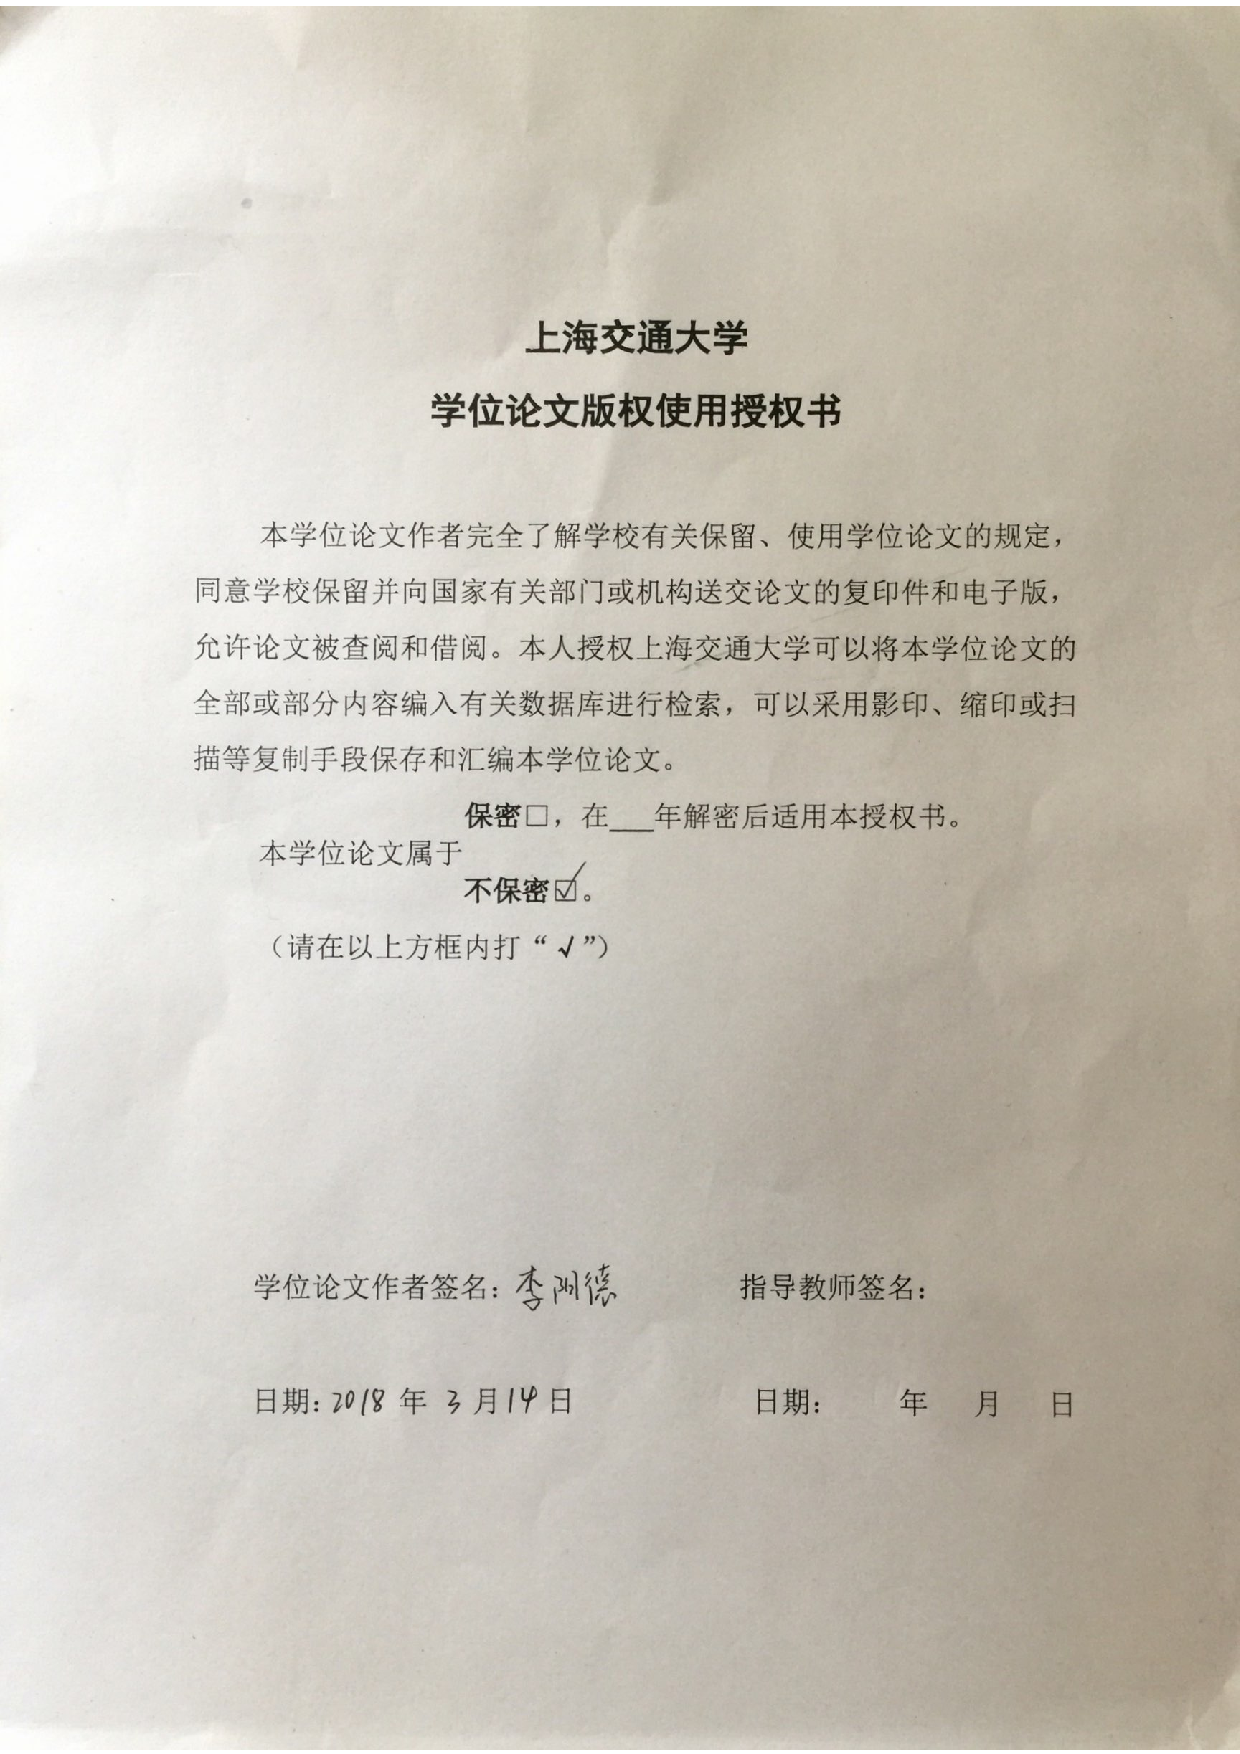
\includepdf{pdf/authorization.pdf}
	\cleardoublepage
\else
\ifsjtu@review\relax
% exclude the original claim and authorization
\else
	\makeDeclareOriginal
	\makeDeclareAuthorization
\fi
\fi
\makeatother


\frontmatter 	% 使用罗马数字对前言编号

%% 摘要
\pagestyle{main}
%# -*- coding: utf-8-unix -*-
%%==================================================
%% abstract.tex for SJTU Master Thesis
%%==================================================

\begin{abstract}
% update at last
网络功能虚拟化(NFV)在云计算基础设施部署时表现出了业界的期待敏捷性和可扩展性,但软件化网络服务的性能仍然阻碍了其普及。云中的大多数网络服务在标准高容量服务器(SHVS)中作为服务功能链(SFC)运行,SHVS由虚拟机(VM)组成。每台虚拟机都在SFC中运行专用的虚拟网络功能(VNF。hypervisor将这些虚拟机作为单个实例运行VNF来维护。当SFC被请求服务时,资源管理器缺少对正在运行的VF之间的连接的细节的识别,并且分开分配资源,从而导致SHVS的低效资源利用。为了解决这个问题,本文提出了一个新的资源抽象考虑链式NFV工作负载的基本特征。我们基于我们的模型设计了一个两阶段算法,叫做\ textbf {Furion}来调度资源分配。该算法在实际IP多媒体子系统(IMS)平台上进行了测试,并与现有的通用方法进行了比较,结果表现出明显的提升。

\keywords{\large 上海交大 \quad 饮水思源 \quad 爱国荣校}
\end{abstract}

\begin{englishabstract}
Network Function Virtualization (NFV) shows agility and scalability in industry when deployed in cloud computing infrastructure, but the performance of softwarized network service still impedes its popularization. Most of the network service in cloud run as service function chain (SFC) in Standard High Volume Server (SHVS), consisting of virtual machines (VMs) in tandem. Each VM runs a dedicated virtual network function (VNF) in SFC. The hyper-visor treats these VM with running VNF as single instance to maintain. When SFC is called for serving, the resource manager lacks the recognition of details on the connections among running VFs and separately allocate the resource which consequently lead to low efficient resource utilization for SHVS. To resolve this problem in this paper, we propose a new resource abstraction considering the chain-style NFV workload with underlying characteristics. We design a two-phase algorithm based on our model called \textbf{Furion} to schedule the resource allocation. The algorithm is tested in real IP Multimedia Subsystem (IMS) platform and compared to existing generic methods, and the result shows obvious enhancement.

\englishkeywords{NFV, SFC, Multi-core Server, NUMA, Mapping, Dynamic Benchmarking}
\end{englishabstract}



%% 目录、插图目录、表格目录
\tableofcontents
\listoffigures
\addcontentsline{toc}{chapter}{\listfigurename} %将插图目录加入全文目录
\listoftables
\addcontentsline{toc}{chapter}{\listtablename}  %将表格目录加入全文目录
\listofalgorithms
\addcontentsline{toc}{chapter}{算法索引}        %将算法目录加入全文目录

%\include{tex/symbol} % 主要符号、缩略词对照表

\mainmatter	% 使用阿拉伯数字对正文编号

%% 正文内容
\pagestyle{main}
\chapter{绪论}
\label{chap: Introduction}
\section{课题主要研究内容及背景}
网络功能虚拟化(Network Function Virtualization,NFV)是由欧洲电信标准组织 (ETSI) 从网络运营商的角度出发提出的一种软件和硬件分离的架构,是当前学术界和工业界十分热门的话题之一。其实质是通过标准化的IT虚拟化技术,采用业界标准的大容量服务器、存储和交换机承载各种各样的网络软件功能,实现软件的灵活加载,从而实现可以在数据中心、网络节点和用户端等不同位置灵活部署。NFV利用标准IT虚拟化技术来加速网络运营商和服务提供商的服务更新,随着近些年来学术界和工业界的携手推进,NFV正在逐步的落地并替代传统的通信服务平台。如今的网络是仍然由各不相同的网络物理设备彼此相连从而实现特定的服务功能,但这样的架构恰恰成为了网络服务更新的掣肘。NFV的目标是使用虚拟的网络功能来替代这些特定的网络设备,在x86等通用性硬件上利用虚拟机化技术来承载大量的网络功能软件,从而降低网络昂贵的设备成本。通过软硬件结构及功能抽象,NFV技术使得网络设备功能不再依赖专用硬件,资源可以充分灵活共享,实现新业务的快速开发,并基于实际业务需求进行自动部署、弹性伸缩、故障隔离和自愈等具体目标\cite{etsi2013001}。

欧洲电信标准化协会(ETSI)作为NFV的发起标准组织,于2015年年初发布了NFV参考架构等系列文稿,虽然ETSI NFV阶段成果不是强制执行的标准,但是得到了业界的普遍认可,已经成为了业界的事实标准。目前NFV的标准框架已得到各方的基本认可,各厂商也基本按照现有的标准架构开发和推进各自的服务框架。如图\ref{fig:NFV}所示,NFV标准框架主要由NFV基础设施(NFV Infrastructure,NFVI)、虚拟网络功能(Virtual Network Functions, VNFs)和NFV管理与编排系统(NFV Management and Orchestration, NFV MANO)三个主要部分组成。其中,NFV基础设施指的是承载具体业务的通过虚拟化技术所管理的数据中心资源。与传统电信机房不同,数据中心具有统一的管理标准和更加普通的x86通用服务器,其维护管理成本和业务升级的成本相较与传统电信业务的中心机房(Central Office)要更加低廉。虚拟网络功能是具体业务的运行实体,结合传统电信的业务支撑系统和管理支撑系统(OSS/BSS)作为上层应用系统,以虚拟化软件的形式,运行在NFV基础设施中,并接受管理编排系统的功能管理。而NFV管理和编排子系统作为衔接IT虚拟化基础设施和传统电信业务的关键系统,收到了众多厂家的重点关注,也是目前研究的重点之一。MANO系统负责解析上层业务、映射并管理具体的物力资源、编排具体业务系统等多项重要业务,其重要性不言而喻。特别是对于底层资源的管理,对于传统电信来说是全新的问题和挑战。目前工业界主要工作仍集中在NFV管理和编排系统开发中,而其中关于通用服务器的性能和可靠性问题仍有待解决。
\begin{figure}[!htp]
	\centering
	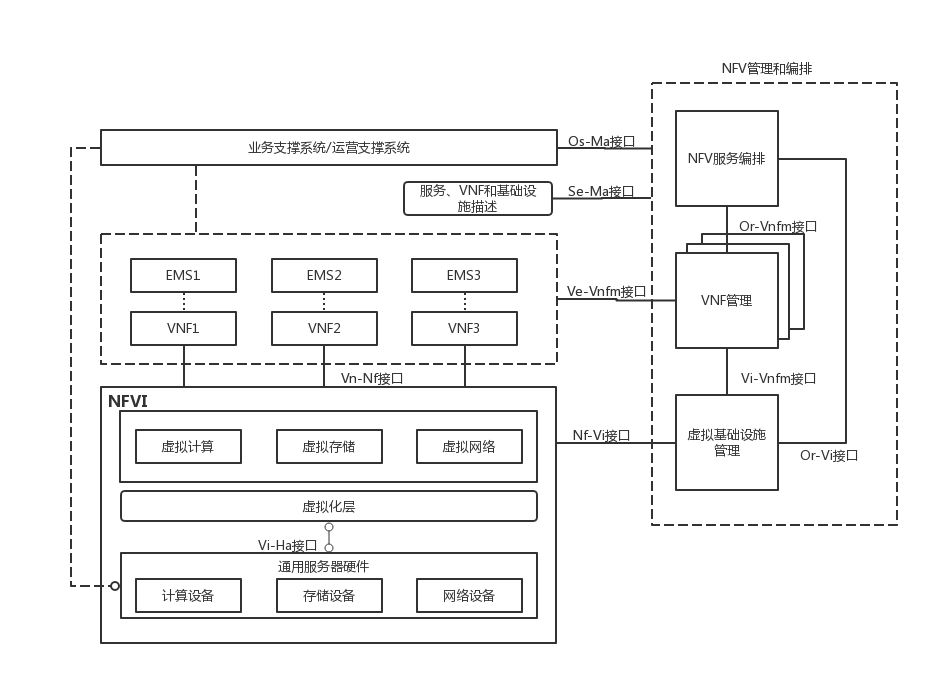
\includegraphics[width=1\textwidth]{ETSI.png}
	\bicaption[fig:NFV]{NFV标准框架}{NFV标准框架}{Fig}{NFV Standard Architecture}
\end{figure}

%为了实现NFV,保证NFV从专门的硬件中迁移到普通服务器中性能和资源分配管理是现阶段学术界和工业界所面对的主要问题\cite{mijumbi2016network}。根据已有的研究总结,当下的通用服务器要面对以下几个NFV环境下的新挑战\cite{hawilo2014nfv}:(1)通信网络中数据面的大负载而带来的性能压力。 (2)电信网络拓扑对管理的严格要求。这些挑战都亟待解决,并且对实现NFV功能落地具有重要意义。

在NFV的众多热点技术中,虚拟化资源调度作为NFV管理与编排系统的核心业务成为了工业界和学术界研究的热点问题。而其中的服务链技术(SFC,Service Function Chain)更是因为其接近实际应用场景的特点,受到广大研究的重点关注\cite{zave2017dynamic,kulkarni2017nfvnice,mijumbi2016network}。在传统网络中,负载均衡器、网关、虚拟防火墙等网络功能共同被称为业务功能点,而流量在经过了一系列处理后,形成了所谓的网络功能服务链。与虚拟化流量调度方式不同,该方式更倾向于对虚拟网络中如何通过控制服务器对网络流量转发进行编程控制,即以更为灵活的方式实现流量到业务功能点的调配和处理。在SFC中,网络的转发效率决定了整体网络的性能,所以如何优化虚拟化资源分配对于提升NFV性能具有重要意义。
	
学术界目前对于SFC的研究主要集中在两方面:(1)优化通用操作系统和网络协议栈,自底向上地提升NFV应用的性能,打破网络服务中来自底层通用平台和通用操作系统的性能瓶颈。(2)提出针对NFV应用的资源分配算法,优化资源分配效率和网络功能服务节点间网络流量的路径规划。

其中,在优化通用操作系统网络协议栈的方向,近些年学术界涌现了一系列的研究\cite{rizzo2012netmap,ram2013hyper,belay2014ix,hwang2015netvm,yasukata2016stackmap,prekas2017zygos},结合工业界提出的高速网络包转发框架DPDK\cite{intel2015data},从简化网络协议栈,重新分配虚拟化资源和减少无关开销等角度尝试优化基于x86服务器的操作系统和虚拟化框架。这些方法都提高了标准通用服务器的网络性能,然而这些研究并未针对实际的NFV应用进行特定的优化,忽略了NFV应用的特有的各网络功能节点组织形式如服务链等,仍然从一般系统软件的角度去提升基础网络性能,针对NFV具体组织形式的底层优化仍然较少。

文献\citen{xie2016service}指出在NFV资源分配问题(NFV resource allocation,NFV-RA)中,如何解决基于NFV网络基础设施的资源分配是一项重要的挑战。进一步的,文献\citen{herrera2016resource}中将该问题划分为更细的粒度进行深入研究,为研究此类的问题指出了具体的研究方向。这类问题与文献\citen{belbekkouche2012resource,fischer2013virtual}所提出的传统网络中的网络功能映射问题 (Virtual Network Embedding,VNE) 相关,已有的研究参照VNE问题的研究成果和NFV背景下的具体问题,提出了一系列与实际应用相结合的启发式算法。有的从网络时延角度出发,如文献\citen{mijumbi2015design}所述,对NFV的部署和映射问题进行建模,给出了基于贪心和禁忌搜索的两种针对虚拟网络功能转发图映射和虚拟网络功能调度子问题的求解。此外,文献\citen{lin2016demand}从网络开销角度出发,提出了基于混合整数线性规划的方法来最小化网络功能的部署和网络流量的路由问题。这些研究都从上层角度结合NFV的应用给出了解决NFV实际应用的思路,但是大部分研究使用仿真的平台进行算法有效性的验证,对于求解问题实际物理平台上的可行性缺乏有力的证明。

\section{国内外研究现状}
本节介绍并讨论与研究课题相关的国内外研究现状与发展趋势,重点包括国内外研究中对网络功能虚拟化中服务链问题的介绍,针对网络I/O优化,NFV资源分配问题,以及国内外研究者在多核架构下针对该问题的一些研究成果。同时,本章中也将本文所设计的优化解决方案与已有的解决方案和处理思路进行对比,对相关研究的研究内容进行比较和优缺点的分析。

\subsection{网络功能服务链}
根据文献\citen{bhamare2016survey}的定义,网络功能服务链是抽象服务功能(Service Function,SF)的有序或部分有序集合,包括对数据包,数据帧和数据流的有序约束分组。由于服务拓扑的复杂性,各个功能节点在服务链中的位置应具有相对的灵活性。文献\citen{quinn2015problem}总结了现阶段SFC研究所面临的挑战,主要包括:(1)复杂的网络拓扑依赖。原有的服务链是在硬件层面实现的,网络功能与底层硬件拓扑是绑定的,因此网络功能的增加与删减需要直接操作硬件,而NFV所带来的虚拟网络功能需要网络管理员最大可能的优化利用现有的网络资源,复杂的网络拓扑会给动态管理网络功能带来挑战。(2)严格的配置管理。服务链的网络功能节点顺序有着严格的要求,错误的服务配置会导致服务失败,严重影响服务质量,因此如何保证服务链的正确配置也是业界重点关注的领域 (3)受约束的服务弹性。服务链复杂的拓扑限制了服务链快速伸缩的弹性,服务链中任何一个网络节点的失效都可能导致服务链的伸缩失败,保证服务链所以功能节点的可用性对实现可扩展的服务链具有重要意义。文献\citen{ghaznavi2015elastic}研究了在弹性网络功能下的服务链放置问题,虽然与传统的网络放置问题相似,但网络功能额外的灵活有序要求对该类问题进行重新建模,并基于新的模型进行求解和优化。本文所研究的网络功能服务链是基于传统的串行服务链,针对服务链所运行的通用服务器平台资源进行建模并优化求解。相比于已有的研究,本文使用更接近实际应用平台的具体NFV业务,并借助虚拟化平台和具体业务平台来具体实现NFV业务,所得出的解决方法和结论更具有代表意义。

\subsection{网络I/O优化}
为了减小在虚拟化环境中运行虚拟机所带来的额外开销,文献\citen{martins2014clickos}对虚拟机操作系统进行了裁剪,使用微内核的方式构建了基于MiniOS\cite{popuri2014tour}的最小化操作系统ClickOS,并在Xen\cite{barham2003xen}的基础上将后端交换机Open vSwith\cite{pfaff2015design}替换为了高速的VALE交换机\cite{rizzo2012netmap},使用Click语言\cite{kohler2000click}进行NFV网络功能逻辑搭建,从而大大减少了虚拟化所带来的性能开销,提升了虚拟机的网络吞吐。但是在小包的测试环境中,该系统出现了剧烈的性能抖动,而且所能实现虚拟网络功能仍处于单个功能节点阶段,尚未组成服务链,并不能满足NFV复杂的业务需求。相比文献\citen{martins2014clickos},文献\citen{hwang2015netvm}基于KVM平台\cite{kivity2007kvm}推出了NetVM,利用了高速的包转发框架DPDK\cite{intel2015data}大大提升了网络协议栈的包转发速率,并通过共享大页内存、零拷贝数据传输以及优化CPU调度器提升了数据在VM之间的传输效率,减少了由于虚拟化中虚拟CPU的调度所引起的上下文切换开销。本文中借鉴了文献\citen{hwang2015netvm}的平台,在KVM基础上使用virtio\cite{russell2008virtio}方式来优化VM之间的网络传输性能,通过优化多核服务器中虚拟机间资源的亲和度关系,解决在SFC的背景下NFV应用的性能优化问题。

文献\citen{panda2016netbricks}针对基于虚拟化技术实现的NFV提出不同的看法,认为基于现有的虚拟化技术 (VM或容器)所提供的隔离性会带来很高的性能开销,并且针对虚拟化来开发相应的网络功能是个十分繁琐的过程,为了减少这类与服务无关的开销,他们提出了一个新的NFV框架NetBricks来解决这两个问题。对于构建NF,文献\citen{panda2016netbricks}使用Rust语言构建了一小组可定制的网络处理元素,利用该语言的类型检查和安全运行机制来提供基于软件的隔离,将网络功能虚拟化与虚拟化框架解耦,使得软件化的网络功能不再依赖虚拟化平台,极大地减少了构建网络功能的开销,从而实现整体I/O性能的提升。文献\citen{panda2016netbricks}所提出的优化思路十分值得借鉴,但是现阶段完全抛开虚拟化框架实现NFV的成本太高,而且现有的虚拟化管理框架所带来的优势并不能体现,这样的做法会使得NFV失去与当前云计算平台相结合的优势。本文依然采用的是基于KVM的虚拟机实现模式,尽管虚拟化会引起较高的开销,但是同时所带来的更加简单的实现方式,以及更好的隔离性保障可以使得我们专注于解决服务链的资源分配问题。


\subsection{NFV资源分配问题}
在NFV资源分配问题方面,文献\citen{herrera2016resource}详细介绍了NFV资源分配问题的研究现状,并总结了资源分配问题的具体子问题,即虚拟网络功能组链 (VNFs Chain Composition,VNFs-CC), 网络转发图映射 (VNF-Forwarding Graph Embedding,VNF-FGE)和虚拟网络功能调度 (VNFs Scheduling, VNFs-SCH)。文章将NFV下的资源分配问题归结为NP-hard问题,并指出了解决此类问题的三种解法思路:确定解法、启发式解法和元启发式解法。具体来讲,针对VNF-FGE问题,确定解法中的整数线性规划方法可以在可接受的时间内给出最优解。而在时间敏感的NFV-RA问题下,确定解法的时间开销超出了预期限制,这时就需要借助基于启发式和元启发式的高级算法来减少算法的运行时间和额外开销。

文献\citen{hsieh2016network}认为在数据中心,网路功能服务链使工作流以特定的顺序遍历不同的网络功能,为其客户提供不同级别的服务。由于服务链中任何相邻网络功能之间的距离将决定该链路的总带宽消耗,那么虚拟化网络功能在数据中心中的放置便成为了影响整体带宽的重要问题。在文献\citen{hsieh2016network}中,这种放置问题被归纳为一个多层背包问题。文献\citen{hsieh2016network}针对树状网络拓扑,文章提出了两种基于贪心的算法:多层最差拟合和多层最佳拟合。在仿真平台的实验结果表明,与传统的最优算法相比,MWF可以将带宽消耗降低15%,而仅使用服务器数量增加1%。	


\subsection{其他相关研究}
除了对于网络I/O的优化和NFV资源分配问题的研究,很多文献和论文也从其他角度对网络功能虚拟化进行了研究。
%TODO MANO框架研究
文献\citen{mijumbi2016management}总结了在网络功能虚拟化管理和编排时可能会遇到的挑战


%TODO 线程调度
文献\citen{hu2016towards}认为当前在使用NFV部署在现代的大通量标准服务器时会面临许多挑战。因为NFV数据平面及其服务功能链的复杂性特征,现代NFV部署在大容量通用服务器上以异构软件流水线的方式呈现。NFV流量必须由异构处理软件组件从NIC到终端接收器。由于流程的端到端性能是合作的由每个处理阶段的性能决定基于NUMA的SHVS中的资源分配/映射方案必须考虑线程依赖调度来折衷影响的共同争用和远程数据包传输。在文章中,他们开发了一个线程调度机制协调放置HSP的线程以最小化端到端NFV交通流量性能下降。它采用动态的基于编程的方法来搜索最优线程映射具有可忽略的开销。为了服务这个机制,我们还开发了一个性能下降估计模型准确估计每个阶段的业绩下滑HSP。实现我们的协作线程调度机制在真正的系统上,并使用真正的工作负载进行评估。平均而言,我们的算法胜过最先进的NUMA aware和竞争意识调度策略至少7%CPU利用率和23%的流量吞吐量可忽略不计计算开销(少于1秒)。

\section{论文安排}
本文对网络功能虚拟化中,虚拟机资源调度进行了研究,论文的具体结构和内容安排如下:

第一章作为绪论,主要介绍了本课题的主要研究内容和研究背景。进一步的对于本研究相关的工作进行了介绍和梳理,主要从网络I/O优化研究和NFV资源分配研究两个角度以及其他相关研究介绍了国内外已有的研究成果。最后本章对全文的结构和安排做了介绍。

第二章重点介绍了与本文的研究紧密相关的研究背景和相关技术,包括NFV的发展历程,目前主流的网络I/O虚拟化技术分类,多核服务器架构已经在多核服务器下的虚拟机性能观测,最后还介绍了本所所使用的具体NFV应用平台Clearwater,为读者了解与研究相关的知识和下文的展开做了准备。

第三章着重介绍了本研究中研究方案的具体设计,包括方案的设计目标,基于服务链的建模,系统的设计思路和系统具体的模块设计等。同时,也依次详细介绍了文本的设计方案的各个子模块的具体设计思路,描述了基于模块设计的系统工作流。

第四章将介绍本研究中的研究方案的具体实现,以总体算法框架为切入点,分模块介绍了本文系统各子模块的实现方法。

第五章从实验的角度对本文的设计进行了性能上的测试。通过利用Clearwater自带的压力测试工具和基础性能测试工具iPerf、Ping、Apache等,在真实的测试环境下对本文所提出的系统进行了严格的测试。

第六章归纳全文,总结和回顾了全文的研究内容和主要研究结论,并提出了一些研究展望。

\section{本章小结}
本章主要整理和归纳与本研究密切相关的国内外研究现状和发展趋势。本章中,重点介绍了国内外的相关研究中,网络功能虚拟化带来的一系列挑战和存在的问题。同时,本章中也对现有解决方案进行了深入的探讨,分析这些方案的共同点和优缺点,与本研究中的设计相对比。本章也对网络功能虚拟化的研究热点进行了介绍,特别是对当前研究较为火热的资源调度问题及相关研究的研究成果进行了简单的归纳和总结。
\chapter{网络功能虚拟化相关技术}
\label{chap:relatedwork}

\section{网络功能虚拟化发展概况}
2012年10月,ETSI的NFV规范小组在德国的达姆施塔特发表了关于软件定义网络(SDN, Software Defined Network)和OpenFlow的白皮书,期间正式推出了NFV概念。自白皮书发表以来,该小组制定了每两年为一个发布周期的工作计划,持续推出更加具体的协议规范和标准术语定义以及NFV的使用案例。截止本文,NFV小组已经进入了第三个发布周期。

在第一个周期2013-2014年内,小组的主要工作目标是:
\begin{enumerate*}[label=\itshape\alph*)\upshape]
	\item 推动网络运营商融合NFV。
	\item 将已有的适用标准纳入网络服务和产品中。
	\item 以促进创新和培育供应商开放的生态系统为目标,同步地开发新的技术规范。
\end{enumerate*}
截止2014年,工作组除了前期发布的6篇定义性文档,又陆续发布了11篇详细的技术规范,包括。。。 第一套文档标志着NFV的标准化初期工作已经完成,需要对划分的各个工作领域进行进一步的详细定义和约束。

第二个周期2015-2016年,小组的工作重心已经转移到了VIM,VNFM,NFVO以及各功能接口的具体定义中。进一步的,在该阶段的工作中,小组还重点推出了适用于当前NFV服务需求的信息模型参考,在模型中预留了解决各项实际问题的参数接口,为各厂商开发自己的NFV服务框架提供指导。各项文档均已在ETSI官方网站发布。

目前,NFV规范小组正处在2017-2018发布周期内。根据已发布的计划,在本周期内他们有23个工作目标,包括20个新功能点和3个对上一周期的已发布文档的补充。在该周期内,小组的工作重点是深入定义核心的NFV信息模型,完善支持NFV非业务子系统接口如计费,账单,用户管理,监管,安全等,以及对MANO服务的多方面支持。同时在近些年来,NFV工作组联合了如Linux Foundation,OpenDayLight等开源社区以及工业界各服务提供厂商,旨在携手推进NFV落地实现,与现有业务平台平滑过渡衔接。他们推出了各种开源的NFV平台如OPNFV,OpenSource MANO,Open-O, Cloudify等等。学术界近年来对NFV的研究也进行得如火如荼,相关介绍在第1.2章节中已有详细的介绍。


\section{常见的网络I/O虚拟化技术}
虚拟化技术作为NFV的基础,是实现NFV的关键技术。I/O虚拟化,特别是网络I/O虚拟化,更是直接影响了NFV性能的关键因素。在本节中,我们将介绍和分析三种主流的网络虚拟化模型:设备仿真模型(Device Emulation),分离驱动程序模型(Split-driver)和硬件辅助模型(Hardware-assisted),并对这三种模型在实际应用场景下做出对比。

\subsection{设备模拟模式}
设备模拟模式是一种通过在虚拟机监视器中模拟敏感指令和特权指令的方式来模拟物理设备I/O操作的全虚拟化实现方式。如图\ref{fig:device_emu}所示。这种模式充分利用二进制翻译技术和直接执行技术的组合来从客户操作系统中抽象和分离底层硬件,实现纯软件方式的硬件仿真。虚拟机操作系统实例和用户级别指令可以在没有感知底层虚拟化环境的情况下不加修改地运行,所以设备模拟模式为I/O操作提供了最佳性能隔离和安全性,简化了客户端虚拟机的迁移操作和提升了其可移植性。工业界有很多成熟的产品如VMware Workstation\citen{} 和VMware ESX Server\citen{} 都支持这种I/O虚拟化的方式。此外,XEN和KVM的QEMU也可以配置支持设备模拟模式的I/O虚拟化。
\begin{figure}[!htp]
	\label{fig:device_emu}
	\centering
	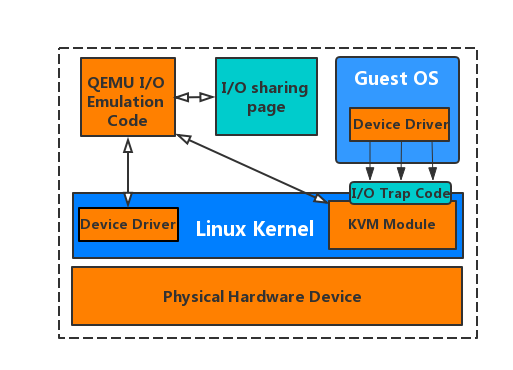
\includegraphics[width=0.8\textwidth]{Device_Emulation.png}
	\bicaption[fig:SRR]{设备模拟模式示意图}{设备模拟模式示意图}{Fig}{Device Emulation}
\end{figure}
但是,这种方法也存在很大的缺陷,由于虚拟机监视器需要动态翻译所有操作系统指令并缓存所有结果,因此虚拟机监视器设备驱动程序一旦发生故障将导致所有客户虚拟机的I/O中断。而且,由于在运行时对这些敏感和特权的指令请求处理需要进行代价高昂的陷入和仿真操作,频繁的此类操作将引起巨大的性能开销,成为影响I/O性能的瓶颈。根据已有的研究,每个I/O操作的陷入和仿真都将导致客户操作系统和虚拟机监视器之间的上下文切换,其成本约为3000~5000 个CPU周期\citen{}。根据已有的研究实验显示,这样的开销显着地降低了近10倍的I/O吞吐量。这一性能瓶颈挑战严重阻碍了将设备仿真方法部署到高性能网络和配备现代高性能网卡(例如40/100 Gbps 网卡)的数据中心中。NFV的应用场景下需要数量众多的虚拟机频繁的使用各自的网络I/O设备,设备模拟的方式并不能胜任该场景下对I/O设备高性能的需求。

\subsection{分离驱动模式}
为了缓解虚拟机监视器参与模拟的高昂开销,Xen团队首先在半虚拟化场景下开发了分离驱动模式(Split-Driver)\citen{}。紧随其后,KVM的virtio\citen{},VMware tool和VM interface\citen{}也支持了在半虚拟化的分离驱动模式。本文以virtio为例,介绍在KVM平台下奋力驱动模式的实现原理。KVM的分离驱动模型如图\ref{fig:split_dri}所示,它由主机中的前端virtio驱动和后端驱动组成。当虚拟机向服务器内的另一台虚拟机发送数据时,虚拟机首先将数据加载到其vring缓冲区中的队列,并修改其描述符表。随后通知KVM产生vm-exit信号,并使用ioeventfd方法允许vHost驱动程序接收来自客户端虚拟机的信号。
\begin{figure}[!htp]
	\label{fig:split_dri}
	\centering
	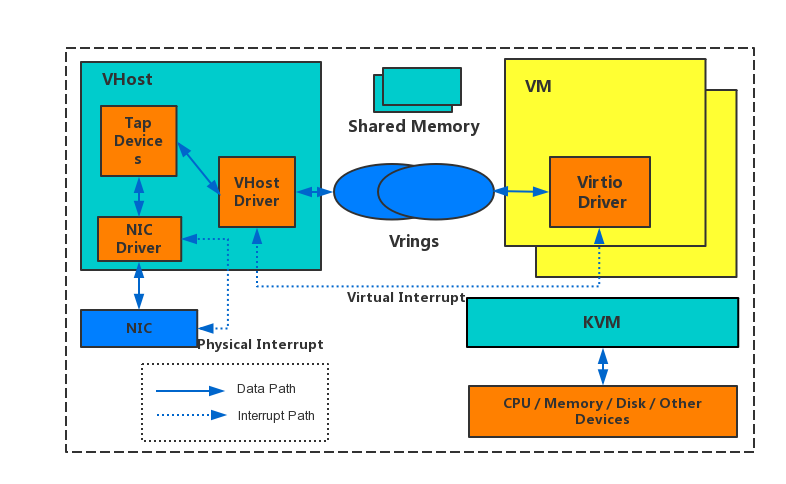
\includegraphics[width=0.8\textwidth]{Split_driver.png}
	\bicaption[fig:SRR]{Split-driver模式示意图}{Split-driver模式示意图}{Fig}{Split-driver Model}
\end{figure}
当vHost驱动获得信号后,前端程序将获取有效队列的物理地址,并将需要传输的数据复制到绑定tap设备地址空间。数据通过网络协议栈被传送到目的地址上。在传送过程中,前端驱动发现如果目标地址是同一台机器上的虚拟机,vHost将利用零拷贝机制,通过共享内存直接将数据的地址指针发送到到目标虚拟机的对应驱动中。当目标虚拟机收到数据后会触发一个回调信号函数,并让虚拟机将传输的数据拷贝放入自己的vring读取队列。总而言之,在分离驱动模式下的虚拟机之间的数据传输可以被看作是将数据从一个内存区域复制到另一块存储区域。分离驱动模式采用高效的I/O通信通道 (I/O Channel) 来避免虚拟机监视器对模拟端口I/O和内存映射功能的干预。因此,分离驱动模式可以利用同样的物理资源达到比设备仿真模式下更高的吞吐量同时降低CPU的利用率。即使半虚拟化方式需要对操作系统内核进行深度修改,无法做到像全虚拟化方式那样对不同客户机操作系统广泛的支持,分离驱动模式还是显示出了其在虚拟机管理和虚拟机迁移方面的巨大灵活性,在当下的虚拟机监视器和虚拟机操作系统中得到了广泛的支持。


\subsection{硬件辅助模式}
设备仿真和分离驱动模式都被分类为基于软件的I/O虚拟化,这种基于软件的模式实现了丰富的I/O设备功能同时简化了对虚拟机I/O设备的管理。然而,这种方式也并不是完美无缺的,纯软件实现方式在面对大量的陷入-仿真操作或者大块数据拷贝的时候会面临高昂的系统开销,这个时候我们可以借助硬件辅助的模式来解决我们的瓶颈。硬件辅助I/O虚拟化模式是为共享本地设备而开发的,它通过继承I/O内存管理单元 (IOMMU) 的用户权限来使用直接I/O技术从而实现绕开虚拟化的内存保护和地址转换,为虚拟机直接分配真实的I/O设备。PCI-SIG工作组针对这种I/O虚拟化的方式制定了规范,通过为每个虚拟机提供独立的内存空间,中断和DMA流来绕过虚拟机监视器直接参与数据处理。特别的,PCI-SIG推出了单根I/O虚拟化 (SR-IOV) 技术,这项技术为针对PCIe设备设计了一组硬件增加技术,通过去除虚拟机监视器在数据包分类和内存地址翻译的干预来实现基于专门硬件的增强。
\begin{figure}[!htp]
	\label{fig:hardware_ass}
	\centering
	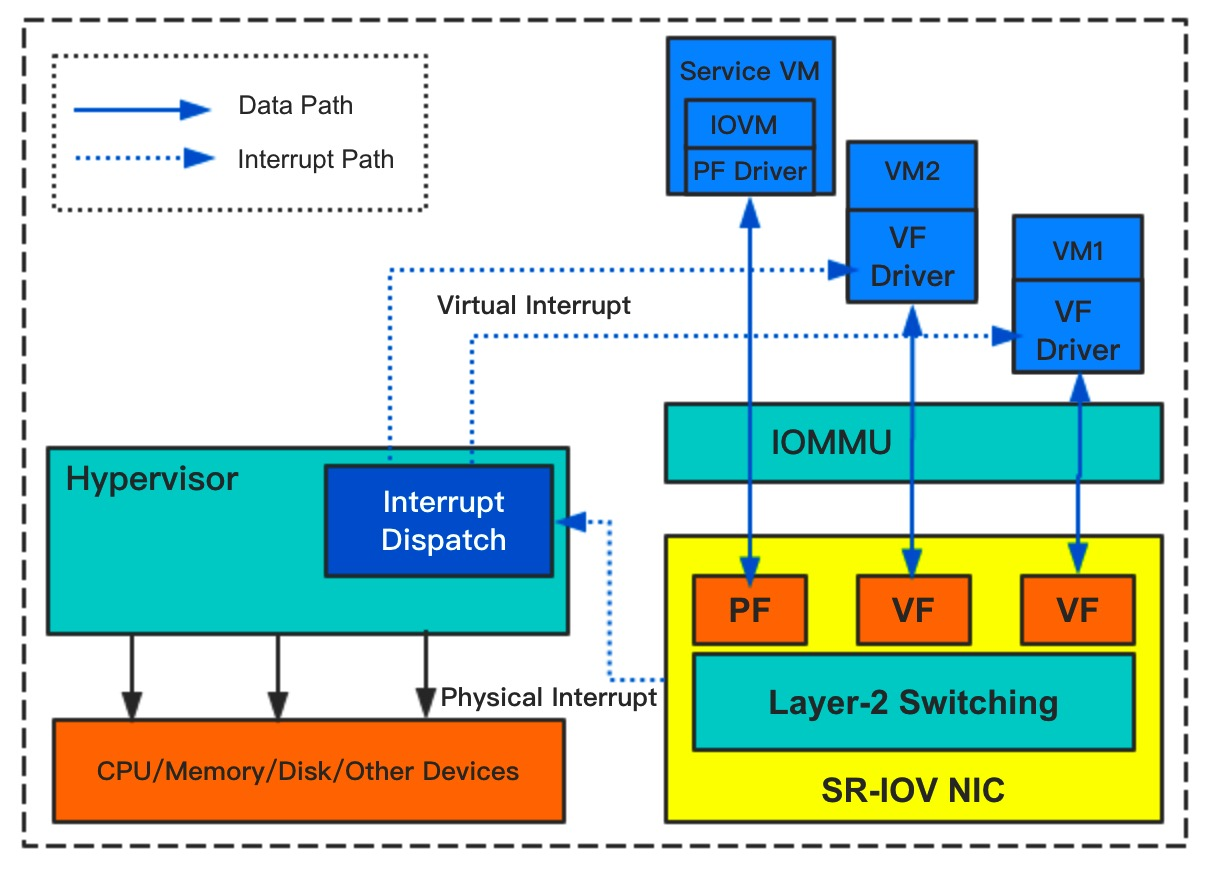
\includegraphics[width=0.8\textwidth]{SR_IOV.jpg}
	\bicaption[fig:SRR]{硬件辅助模式示意图}{硬件辅助模式示意图}{Fig}{Hardware-assisted Model}
\end{figure}
SR-IOV虚拟化模式结构如图 \ref{fig:hardware_ass}所示,一个支持SR-IOV功能的设备可以由虚拟机监视器分配多个虚拟设备(VF, Virtual Function),以普通PCI设备的身份被分配PCI地址空间。宿主机中的物理设备(PF, Physical Function)的驱动程序负责管理和配置VF,而在被分配VF的虚拟机操作系统中,驱动程序将其当做普通的直接分配的物理设备来使用,通过IOMMU直接访问自己专有的VF。通过这样的方式,SR-IOV可以绕过虚拟机监视器实现数据的传递,从而减少移动数据的开销,在降低CPU利用率的同时,减少系统的延迟并挺高网络吞吐量。但是需要指出的是,这种硬件辅助的方式需要手动进行虚拟网络功能的配置,无法实现像软件实现方式那样灵活的迁移和扩展。并且一块PV所能分配的VF是有上限的,这也从硬件角度限制了硬件辅助方式的在多虚拟机应用场景下的应用。


\section{非一致性存储访问架构}
众所周知,NFV的目标是在大容量的标准通用服务器上运行传统通信业务,而现在通用的标准服务器基本都是遵循非一致性存储访问架构(NUMA, Non-Uniform Memory Access)的服务器阵列,为了更好地完成NFV到通用服务器上的迁移,了解通用服务器的基础架构十分必要。图\ref{fig:numa}所示的是Intel Haswell架构下多核处理器示意图,在NUMA服务器中每个处理节点(Socket/Die)与通过内存访问控制器(MC,Memory Controller)与相邻的内存直接相连。同一个处理节点中的多个物理核拥有自己独占的L1/L2级缓存并且通过节点内部链路通道共享L3缓存,内存访问控制器以及PCI-e接口。在一个处理节点内部的的数据传输是通过点对点的高速数据通路 (例如Intel的QPI) 传输的。除了同一个节点内通信,不同的节点间也由相同的高速数据通路相连,不同的处理器节点要访问别的节点的内存时,需要通过内存控制器进行远程访问。
\begin{figure}[!htp]
	\label{fig:numa}
	\centering
	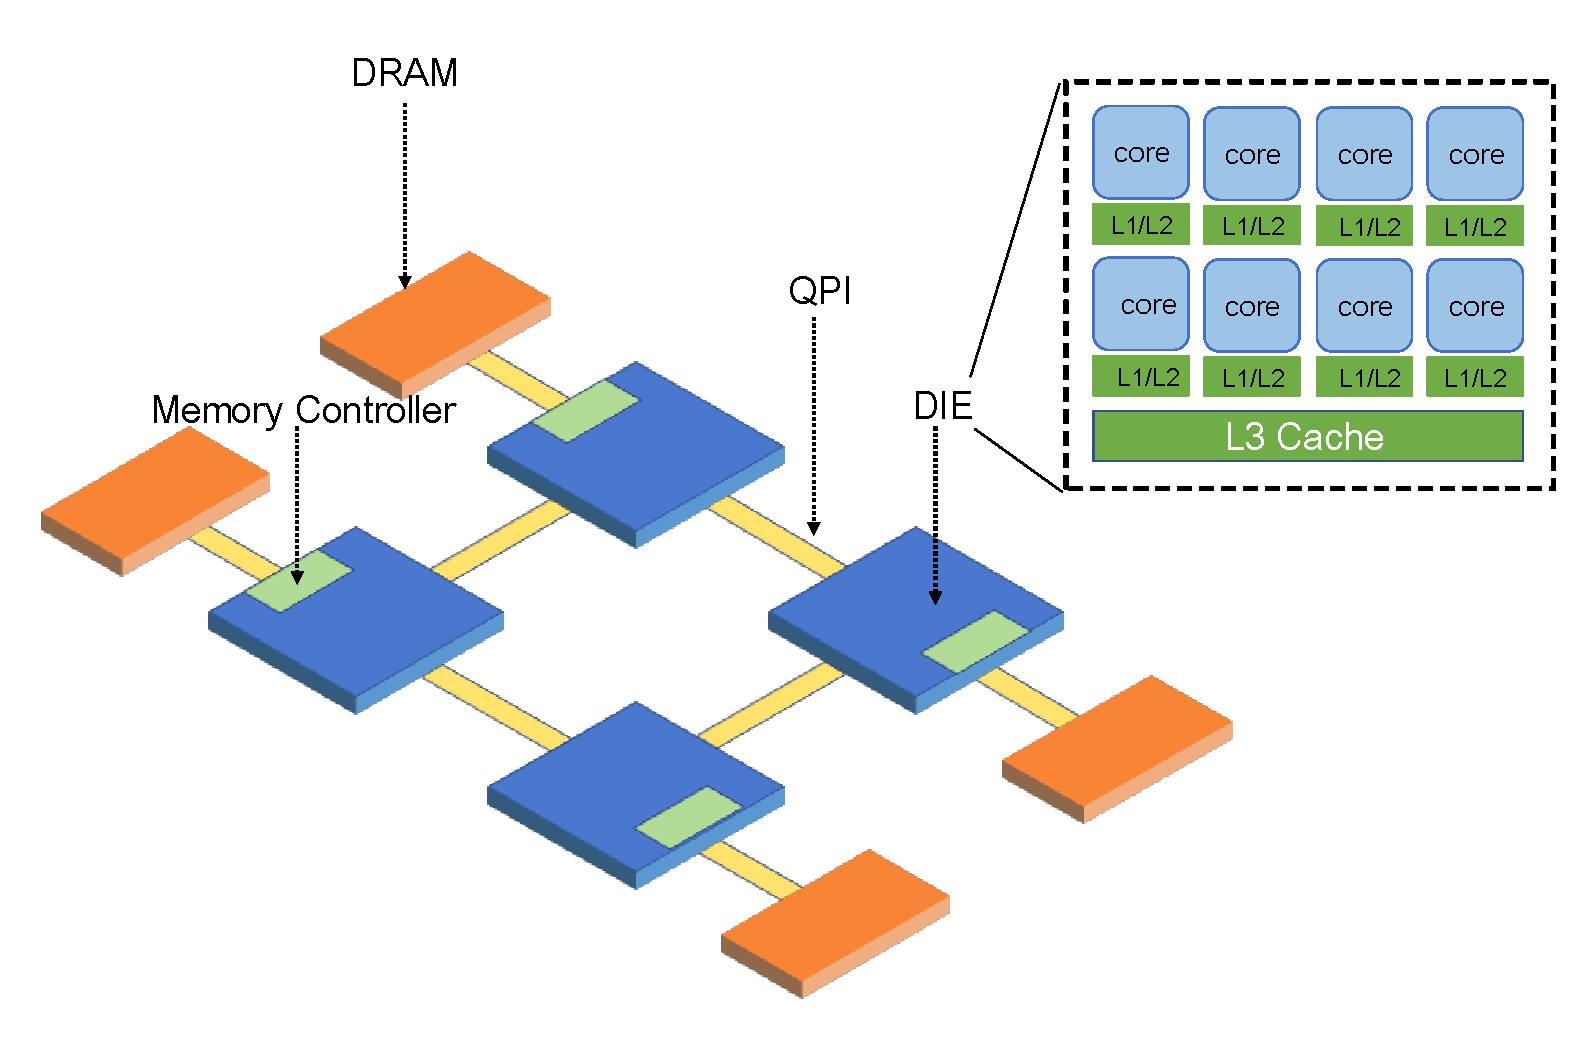
\includegraphics[width=0.8\textwidth]{numa.pdf}
	\bicaption[fig:SRR]{Intel Haswell架构非一致性存储访问示意图}{Intel Haswell架构非一致性存储访问示意图}{Fig}{NUMA Architecture}
\end{figure}
在NUMA架构下,本地和远程内存访问由于机制的差异存在性能上的差异,而节点内共享的内存控制器在竞争过高的情况下也容易成为性能瓶颈导致内存访问性能的剧烈下降,所以如何针对多核通用服务器下非一致性访问的特性来优化应用一直是学术界所面对的经典挑战之一。NFV应用迁移到多核服务器中,不可避免地会遇到NUMA架构所带来的问题,而SFC的服务组织形式下同一条服务链上的虚拟机彼此之间存在大量的数据拷贝传输,如何处理好基于物理架构的物理资源对实现高性能的NFV具有重要意义。
\begin{figure}[!htp]
	\centering
	\subfigure[Netperf带宽测试]{
		\label{exp:netperf_bandwidth}
		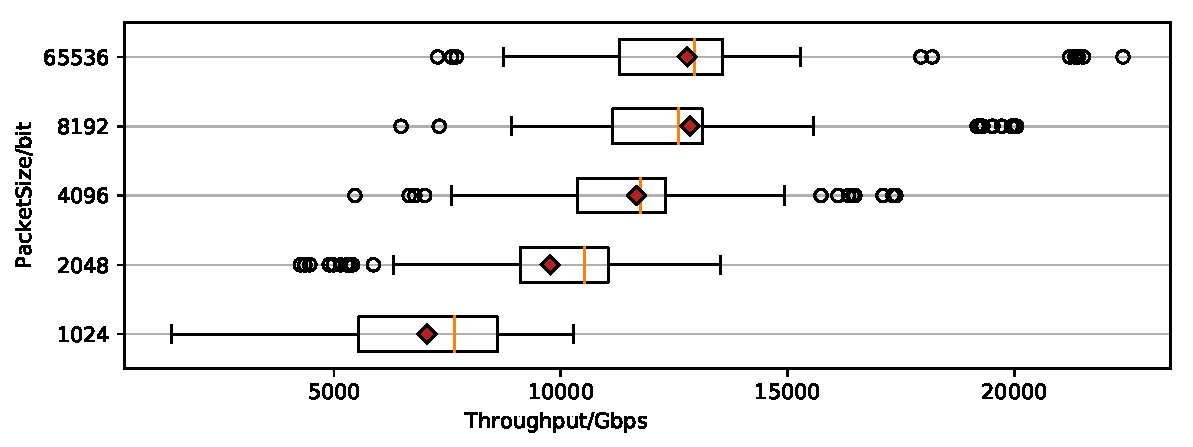
\includegraphics[width=0.8\textwidth]{observation/box1.pdf}
	}
	\subfigure[Httperf带宽测试]{
		\label{exp:httperf}
		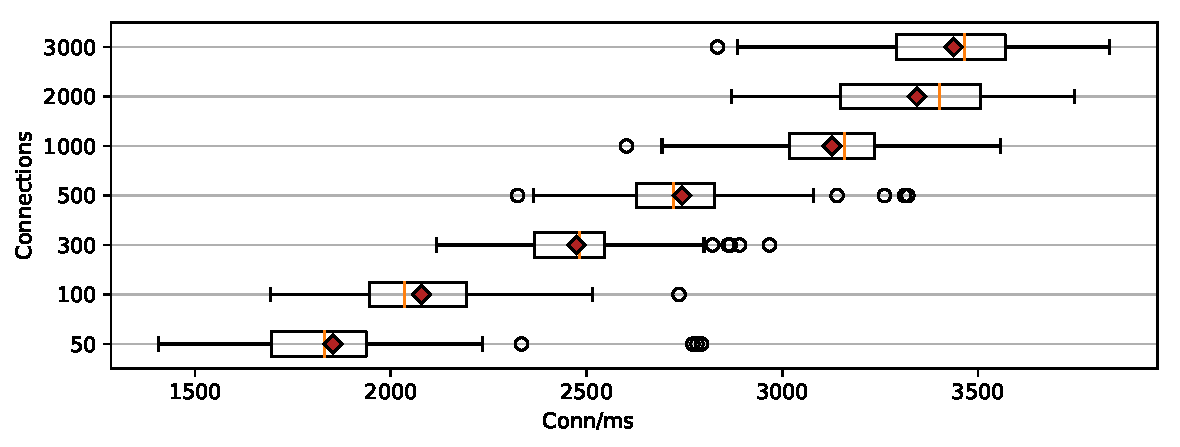
\includegraphics[width=0.8\textwidth]{observation/box2.pdf}
	}
	\subfigure[Netperf延迟测试]{
		\label{exp:netperf_latency}
		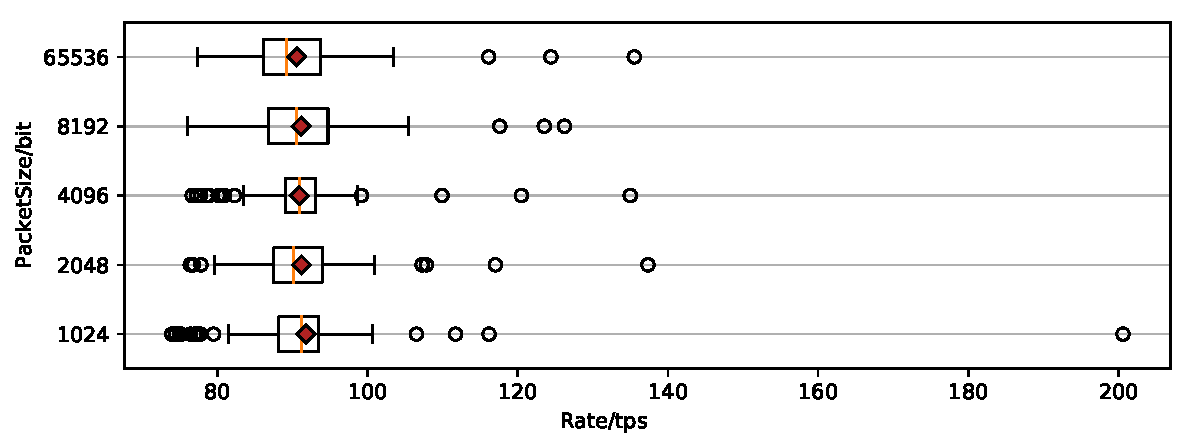
\includegraphics[width=0.8\textwidth]{observation/box3.pdf}
	}
	\bicaption[exp:observe]{模拟应用性能观测结果}{模拟应用性能观测结果}{Fig}{Application Performance Observation}
\end{figure}
\section{多核物理机性能观测与分析}
在多核物理机中,由于存在非一致性存储访问架构的影响,传统应用都针对了NUMA问题进行了对应的优化,如经典的NUMA-aware的线程调度器numad以及已经集成进Linux内核的AutoNUMA Balancing机制。在NFV应用的场景下,网络功能单元是以虚拟机的形式存在,节点间的数据传输实质上是虚拟机利用网络虚拟化的技术进行通信。从服务器硬件的角度看,可以当做一个虚拟机线程向另一个虚拟机线程拷贝或者接收数据。那么在这样的前提下,虚拟机线程所分配的物理资源之间的亲和度关系对虚拟机线程间通信的性能就造成影响。为了验证这一想法,我们在一台通用服务器上进行了模拟NFV应用的的测试。测试平台具体参数见实验部分的表\ref{tab:configure},使用的虚拟化平台为KVM,网络虚拟化方式为Virtio。我们选取了Netperf和Httperf两个基准测试工具,分别模拟微观的数据包负载和宏观的应用负载下来测试性能表现。实验使用两台虚拟机,其中一台固定在一个处理器节点上并绑定本地内存作为虚拟机的分配内存,而另一台虚拟机则不断更改所绑定的物理核及内存,以所有绑定情况作为测试样本,测试的结果如图
\ref{exp:observe}所示。

我们使用盒图的方式来展现模拟应用性能测试观测结果,分别观测了微观下数据包带宽和延迟以及宏观下网络应用应用的测试结果。根据观测不难发现,在分配了相同的物理资源下,不同的资源亲和度情况下性能结果分布的离散程度很高,数据盒的宽度较大并且有大量的离群点出现,离群点之间的观测值差异甚至达到了接近三倍的差距如图\ref{exp:netperf_bandwidth}所示。根据这样的测试结果,我们认为针对虚拟机物理资源间的亲和度来优化服务链中的资源分配是十分必要的。

\section{Clearwater平台介绍}
%TODO整理语句
目前全球的运营开发商都在加速商用的VoLTE开发,多媒体子系统 (IMS)是4G VoLTE商用组件之一,因此也引起了工业界格外的重视。NFV兴起以来,工业界纷纷在尝试将IMS系统部署在NFV平台环境中,探索IMS应用场景在NFV生产环境中的实现,希望能够利用虚拟机技术加速电信业务的研发和部署,降低业务升级的成本和周期。根据我们的调研,在开源的IMS系统领域,有两个十分知名的项目:Clearwater\footnote{项目由Metaswitch Networks 提供赞助,官方网址为 http://www.projectclearwater.org/ }与Kamalio\footnote{https://www.kamailio.org/w/}。而在这两者之中,ClearWater系统更是因为其为云计算平台量身打造的多媒体子系统定位而广受众多厂商和研发人员的欢迎,开发社区十分火热,产品也在迅速的迭代中。它采用大型互联网软件架构的设计思路,以微服务的方式设计各个组件,使得系统本身具有很好的伸缩能力,成为了一个电信级别的开源IMS系统。
其分布式版本的系统架构图如图\ref{fig:clearwater}所示,可以看出该系统主要有三个核心的组件,Sprout,Dime,Vellum和其他边缘组件组成。其中,Sprout节点作为注册和权限管理的路由代理,主要负责处理客户端的认证和应用服务器ISC接口的通信。Sprout节点还包含内置的MMTEL应用服务器,在运行过程中Sprout不负责存储任何持久化的数据,而是通过http协议到Homestead和homer服务中读取HSS的配置信息,如用户信息和MMTEL服务配置等;通过远程调用接口从Vellum中获取用户的注册信息和当前状态等。Dime节点主要负责运行Homestead和Ralf服务,包括对HSS信心的缓存等。而Vellum服务则负责存储各种持久化信息,包括用户的注册注册信息,当前服务的始终状态以及各种权限和密钥等。
\begin{figure}[!htp]
	\centering
	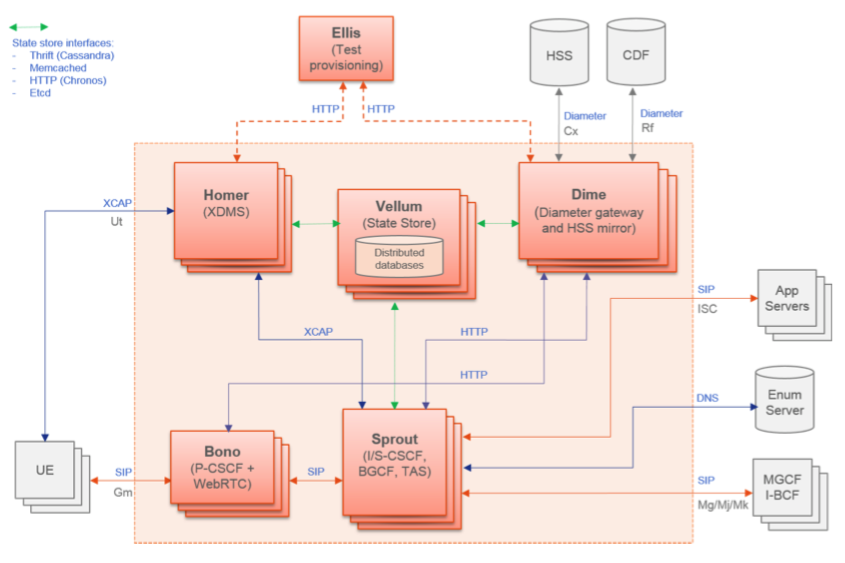
\includegraphics[width=1.0\textwidth]{clearwater/clearwater_arch.png}
	\bicaption[fig:clearwater]{Clearwater系统架构图}{Clearwater系统架构图}{Fig}{Clearwater Architecture}
\end{figure}
Clearwater是针对云计算数据中心开发的IMS系统。众多大型电信运营商纷纷采用基于IMS的标准架构作为其IP语音通话、视频和消息服务的基础构建,用以取代基于传统电路交换系统的上一代VoIP业务系统。Clearwater遵循IMS架构原则,实现了IMS核心网络所需的所有关键标准化接口。有别于别的IMS实现,Clearwater是从云计算作为基础设施的角度设计的。通过结合已在许多全球Web应用程序中验证过的设计模式和开源软件组件,Clearwater实现了前所未有的大规模可扩展性和卓越的成本效益的组合。

\section{本章小结}
本章主要介绍了与网络功能虚拟化技术已经本课题相关的一些技术背景。首先,本章简单总结了下网络功能虚拟化的发展历史和当前的发展现状,介绍了网络功能虚拟化出现的背景,包括与网络功能虚拟户实现相关的虚拟化技术以及多核服务器的架构背景。通过多核服务器的性能观测实验说明了网络功能虚拟化在多核服务器中实现索要面临的实际问题。最后本章着重介绍了本研究所基于NFV实际应用平台Clearwater,包括其业务功能简介和基本架构介绍。
\chapter{方案设计}
\label{chap:design}
本章重点介绍底层平台感知的高性能NFV平台实现的系统设计。在系统初始化过程中,将动态性能测试的结果作为运行时参数输入系统,后续算法将以该参数作为算法执行时的参照标准。当系统收到一个服务链的请求后,需要根据当前可用的系统资源余量进行判断是否响应,并将上层抽象的业务需求转化为具体的服务链业务链表,系统的映射模块根据服务链的逻辑链表来映射相应的具体实例。在映射实例的过程中,本设计所基于的平台所使用的是随机映射的策略,而这种策略在实际的运行环境中缺乏对底层资源的感知,本设计通过对底层物理资源建模并针对性的提出基于资源亲和度的映射策略,从而提升资源的利用效率。

\section{基于服务链的分析建模}
在虚拟话环境中为NFV应用分配物理资源这个问题可以进一步地划分为两个子问题:(1)虚拟机到物理机的映射问题 (2)在已创建的虚拟节点上映射和调度虚拟网络功能。第一个问题已经有大量的研究来解决,本文主要针对SFC前提下的网络功能映射和调度问题。进一步的,为了在实际场景中解决此问题,我们需要对该问题的前提做一些约束。本文所解决的问题基于以下的假设:
\begin{enumerate}
	\item 每个虚拟机实例仅运行一种特定的网络功能应用。网络功能与虚拟机存在多种多样的映射关系,其中,一对一的这种映射关系目前成为了主流。随着轻量级虚拟机的出现\cite{martins2014clickos,manco2017my},一台物理机上所能承载的虚拟机数量得到了极大地提升,因此这种单一虚拟机单一网络功能的模式可以实现复杂的NFV应用。
	\item 每个虚拟机应当专注于处理本身运行的NFV负载,并且尽量避免由于其他无关业务所带来的性能开销。因为我们选择了单核虚拟机并绑定了虚拟CPU到特定的物理CPU从而减少多核调度所带来的额外开销以及上下文切换。
	\item 针对每种特定的网络功能,都有类似资源池的运行实例群组来保证资源的可用性和可扩展性。
\end{enumerate}

\subsection{关键建模定义}
\textbf{网络功能域}{ }考虑到云计算场景下,各种资源都聚合以资源池的方式对外提供,在NFV场景下也不例外。我们以$D$来表示某种特定网络功能的资源池,也称为网络功能域。

\textbf{服务链}{ }我们用$S$代表一条被映射到具体网络上的网络功能服务链。$S$由一群有序的虚拟网络功能组成$S = \{f_{a} \to f_{b} \to f_{c}\}$,其中,$f$是从特定的网络功能域中选取的运行实例。网络流量根据服务链的连接顺序,依次通过每一个功能节点。

\textbf{多层级映射}{ }如图 \ref{fig:mapping} 所示,除了从SFC描述的抽象逻辑服务链到实际运行的网络功能域中运行实例的映射关系之外,还存在着潜在的从服务链到物理资源的映射。我们用集合$N = \{1,...,n\}$ 来表示一台物理机上所有的物理节点,集合$M = \{1,...,m\}$表示一台物理机上所有的物理CPU,根据CPU所处的物理节点,可以将$M$进一步的划分为$ \{\{1,..m_{1}\},...,\{m_{n},m\}\}$。当服务链与运行实例绑定后,服务链与底层物力资源的映射也随之建立。由于虚拟化软件栈的存在,上层的服务链对于所绑定的底层硬件信息并不知晓。但是实际情况是,如同第 \ref{related:observe} 章中验证性实验所示,底层资源之间的亲和度关系对于整条服务链的性能影响相当严重,所以提升服务链的底层资源亲和度对提升服务链的整体性能具有重要意义。
\begin{figure}[!htp]
	\label{fig:mapping}
	\centering
	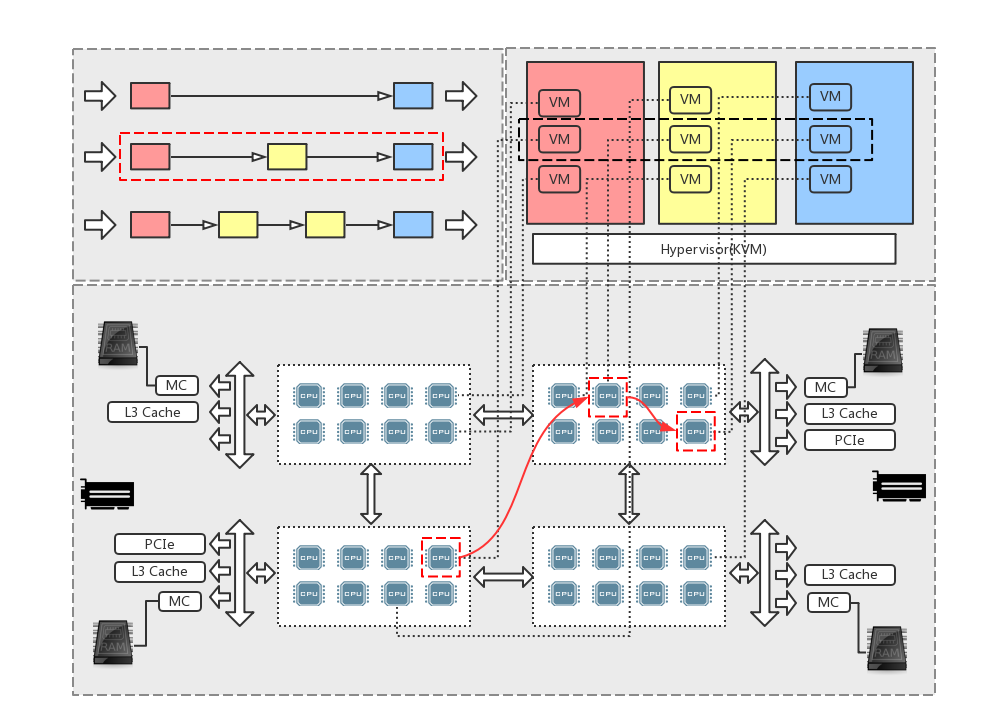
\includegraphics[width=0.8\textwidth]{core.png}
	\bicaption[fig:mapping]{多层级映射关系示意图}{多层级映射关系示意图}{Fig}{Hierarchical Mapping}
\end{figure}

因为NFV中主要的负载是数据流量,所以本文使用衡量网络流量的延迟和带宽参数来衡量NFV的网络性能。我们令 $B_{ij} (i,j \in D, i \neq j)$来表示任意两个运行实例(虚拟机)的的网络通信带宽,令$L_{ij}(i,j \in D ,i \neq j)$ 来表示两者之间通过真实或者虚拟网络通信的网络通信延迟。按照本文的假设,所有的虚拟机仅配置单个物理核,那么显然也存在一个从$f \in D$ 到 $m \in M$的映射。对于服务链上每个虚拟机来说,数据流量将按照串行的顺序沿着数据路径依次通过每个虚拟网络功能节点。为了衡量整个服务链的带宽和延迟,我们需要分析任意两个相连的两个实例之间的带宽和延迟。对于带宽而言,根据串行系统的特性,我们选取整个数据链路上最小带宽作为整条链的带宽值如公式 \ref{equ:bandwidth} 所示。
\begin{equation}
\label{equ:bandwidth}
Bandwidth(S) = \min{(B_{i j } )}  
\end{equation}
对于延迟来说,我们定义了$L(i,j) = L_{i,j} + L_{i} + L_{j}$。其中,$L(i,j)$ 表示数据流量通过以$i$为起点,$j$为终点的服务链的整体延迟,而$L_{i,j}$定义如上文所示表示两个实例的网络传输延迟,$L_{i}$$L_{j}$则分别表示虚拟网络功能处理相关流量而产生的延迟。对于任意一个特定的虚拟网络功能,如果配置了相同的物理资源,则其处理相同网络流量所花费的时间是相同的,也就是说所产生的这部分的延迟是一个固定的值,如公式 \ref{equ:latency} 所示,则服务链上累计的数据流量处理延迟为与服务链业务相关的常数。但是$L_{ij}$这部分的延迟则由于不同物理资源的组合,存在着很大的变化空间。总的来说,服务链 $S$ 上的传输延迟 $L(i,j)$,主要取决于$L_{ij}$。
\begin{equation}
\Delta Latency(S) = \sum_{i=0,j=i+1}{L_{ij}} 
\end{equation}
\begin{equation}
\label{equ:latency}
\begin{aligned}
Latency(S) & = \sum_{i=0,j=i+1}{L(ij)} \\
& = \sum_{i=0,j=i+1}{L_{ij}}  + C \\
& = \Delta Latency(S) + C  		  \\ 
\end{aligned}
\end{equation}

\subsection{网络服务约束及优化目标}
基于上文中已有的模型,这里我们进一步定义模型中的约束和优化目标,包括服务收益,服务开销,和最终优化目标。


\textbf{服务收益}{ }一个服务链的服务收益 $P$ 可以被定义为通过一定的映射和调度策略下从所使用的物理资源中收获的定量的服务。参照已经由公式 \ref{equ:latency} 和公式\ref{equ:bandwidth} 定义的带宽和延迟,总体的服务收益可以被视为这两个指标的线性叠加和,其中 $\alpha$ 和 $\beta$为线性表达式的滑动因子,由服务的具体需求来调整。例如,对带宽要求要求的服务则$\alpha$的值较大,而对延迟敏感的应用则有较大的 $\beta$ 值。

\begin{equation}
\label{equ:profit}
P = \alpha*Bandwidth(S) + \beta* Latency(S)
\end{equation}

\textbf{服务开销}{ }我们从所使用的物理资源的角度来定义一条服务链的服务开销。服务链中的运行实体主要是虚拟机,而对于虚拟机而言主要的资源开销为物理CPU,内存,虚拟硬盘和所分配的其他虚拟I/O设备。在本文中,虚拟硬盘和其他虚拟I/O设备与所研究的主题无关故不做考虑。所以,服务开销 $C$ 定义如公式 \ref{equ:cost} 所示。
\begin{equation}
\label{equ:cost}
C = \delta * \sum{CPU} + \theta *\sum{MEM} 
\end{equation}
公式中的 $\alpha$ 和 $\beta$ 分别是做为根据不同需求NFV应用来调节CPU和内存权重的系数。在本文中,结合本文使用的实际应用,我们令 $\delta = 10^{6}$,$\theta = 0.001$ 。从以上定义不难看出,实际的服务开销和服务收益的主要区别在于实际收益中只计算了数据流量在网络功能节点中的处理时间,而实际服务开销则包涵了服务链在传输线路上的传输延迟。

\textbf{优化目标}{ }从一台通用服务器的角度出发,其所拥有的物理资源是有限的,这就意味着所有运行在一台服务器中的服务链的服务开销 $C$ 的和是有上限的。在这样的前提下,为了能够最大化一台服务器的物理资源利用率,我们需要在开销一定的情况下,尽可能地提升服务收益。我们将最终的优化目标设置为 $T$,如公式 \ref{equ:target} 所示,$T$ 为 $P$ 与 $C$ 的累计和之比,即在有限的物理资源的前提下,通过优化的映射策略尽可能的提升服务链的服务收益之和从而达到最大化 $T$ 的最终目标。
\begin{equation}
\label{equ:target}
T = \sum P / \sum C  
\end{equation}

\section{总体设计目标}
数据从一个网络功能节点传输到另一个节点的过程中不可避免的会产生数据处理和传输的延迟,同时物理带宽同样限制着服务理论带宽上限。在标准的工业生产环境中,单个处理器节点中的物理核数量和内存空间也是有限的,同时通用服务器上不平衡的负载分布也会导致剧烈的资源竞争甚至导致意想不到的性能下降。因此,相比于随机的策略,我们需要相对优化的NFV资源映射和调度策略。在本文中,我们的设计主要关注以下是三个目标:
\begin{enumerate}
	\item 物理资源的实际带宽应当满足服务链的最小带宽需求。
	\item 物理资源的数据传输延迟应当小于服务所允许的最大延迟要求。
	\item 物理资源的整体利用率应当得到保证。一个有效的资源映射策略应当可以保证尽可能的使用可用的物理资源,并在相同的物理资源的前提下提升服务的性能。
\end{enumerate}

\section{总体设计思路}
鉴于已有验证性实验的观测结论和以上对此类问题的目标分析和模型建立,本文所设计的系统需要满足实际NFV应用的最小带宽和最大延迟要求,同时在保证服务质量的前提下提升物理资源的整体利用率。

为了实现以上的设计目的,本系统提供了一种基于底层多核运行平台架构感知的虚拟化网络功能的映射方法。在本系统的设计结构中,当NFV平台得到一个服务请求时,会根据服务请求的解析调度虚拟机资源来组织服务链并提供服务。首先NFV管理平台会评估当前服务资源是否满足提供服务的最小需求,即组成服务链的不同功能域中是否有足够的运行实例。当资源充足时,系统开始根据服务链的实际服务数据流转发图来组织服务。在挑选具体服务实例时组成具体SFC时,系统根据预先处理生成的物理资源亲和度矩阵作为调度算法的输入,根据矩阵中每种资源的亲和度大小关系,依照SFC链的连接顺序,使用局部最优的方法搜索构造出最优的服务链与实例的映射关系,最终结果则交由实际映射模块去从虚拟机角度来实现。

从整体架构上分析,实现基于底层多核运行平台的架构感知的虚拟机化网络功能的映射方法,即本文中所设计动态映射系统包括以下关键步骤:

步骤1、对底层平台进行预处理,获得与平台底层运行时相关的信息矩阵。与普通从硬件中读取参数不同,通过动态采样的方法获取平台运行时实时性能参数能更加准确地反映底层平台的架构差异以及所引起的性能差异。首先,动态采用可以实现与操作系统无关,不管多核平台运行的是什么系统,内核是什么版本,不会影响采样程序的运行结果。其次,相比于直接从主板芯片中读取多核架构中不同处理器节点的粗粒度的亲和度信息,动态采样的方法通过动态地运行测试程序,可以获得更加接近实际情况的量化数据。基于这样的数据信息,我们可以更加准确地刻画底层物理资源之间的细粒度的亲和度信息。最终信息被存进格式化的信息矩阵中,作为步骤2的输入。 

步骤2、当一条服务请求到来时,分析该请求所对应的服务链。根据请求所对应服务链的数据流向确定所需要的虚拟网络功能服务点,并依照信息矩阵中的参数大小来确定待映射的具体运行实例,使用基于贪心的方法生成映射决策序列,进入步骤3。

步骤3、根据步骤2生成映射的实例序列,依次检查实例在对应的物理资源节点当前的负载情况,如果某一实例所在节点的负载过高,增加负载会加剧资源竞争导致当前运行实例的性能下降,则返回步骤2将本次的映射序列标记为失效,重新生成新的实例映射序列。检查通过后进入步骤4。

步骤4、根据生成的映射序列,更新默认的随意选取策略,将备选中的实例的Hostname绑定在域名解析服务器中,实现服务链到实际物理资源的映射服务。

步骤5、当服务链服务生命周期结束时,修改域名解析服务器中的记录,重置服务实例状态为待机中,释放实例资源。


\section{模块设计分析}
\subsection{现有的服务链映射策略}
本文的高性能优化系统基于现有的NFV应用平台 Clearwater 来实现。Clearwater的具体架构与模块相关介绍参见第 \ref{intro:clearwater} 章。在语音和多媒体业务的具体实现中,Clearwater利用云计算资源池化的优势,将各关键网络功能节点以资源池的形式部署在云计算环境中,使用域名解析服务来管理各功能节点之间的连接。默认的服务链实例映射使用随机选取的策略,即根据已有的资源随机选择参与服务组链的运行实例。这样的服务链映射方式随便生成方便管理简单,但是完全忽略了服务链链式服务的数据传输特性,也完全没有考虑底层运行平台的架构差异和资源亲和度信息。同时如果个别处理节点出现负载过高的情况,原有的策略也没有有效的解决方法,甚至有可能加剧某个节点资源竞争,导致服务性能下降的后果。
\subsection{基于底层信息感知的模块设计}
基于对现有平台默认映射策略不足的研究和分析,我们设计了一套底层运行平台感知的高性能NFV系统,该系统架构如图 \ref{fig:system} 所示,想比于原来的服务链映射方式,我们添加了三个模块来实现我们设计目标,即底层信息采样模块 Hardware Sampler,服务链分析模块 Service Analyzer 和动态映射模块 Dynamic Mapper。从图 \ref{fig:system} 中可以看出,我们的系统类似一个中间垫片插入到已有的NFV服务中。上层的业务系统根据具体业务发出服务链服务请求,由管理系统将服务请求下发,服务链需求分析模块收到服务请求后根据具体业务分析出所需服务链,形成组网链表并传递到动态映射模块中。动态映射模块收到服务链表后,根据底层信息采样模块预先生成的信息矩阵生成映射策略,并修改操作域名解析记录来实现组链。
\begin{figure}[!htp]
	\label{fig:system}
	\centering
	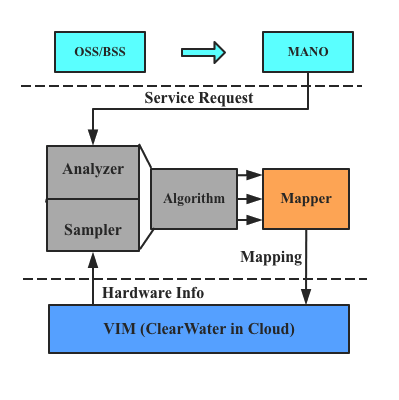
\includegraphics[width=0.7\textwidth]{system.png}
	\bicaption[fig:system]{系统架构示意}{系统架构示意图}{Fig}{System Overview}
\end{figure}
\subsubsection{底层信息采样模块}
在系统架构示意图中,底层信息采样模块负责从底层硬件获取运行平台架构信息和运行时各节点细粒度的性能信息。通过预处理采样等手段,该模块将获取的硬件信息以信息矩阵的方式存储下来做系统输入。

\subsubsection{服务链分析模块}
该模块负责在运行时获取并解析上层业务的具体服务请求,将服务请求转化为特定的服务链链表传递给动态映射模块。当特定的服务链链表生成之后,该模块会检查当前运行系统中的资源余量来确定是否响应服务请求。

\subsubsection{动态映射模块}
基于现有的NFV服务平台,我们利用域名解析实现我们的逻辑服务链到实际链路的映射。当动态映射模块收到服务链分析模块传来的特定服务链链表之后,会根据本文提出的基于贪心的算法来生成与逻辑服务链链表相对应的具体实例链表。这里,我们会根据具体实例所在处理节点的实际负载来确定是否重新生成策略。

\section{本章小结}
本章主要介绍了底层平台感知的NFV平台实现方法的设计结构,包括基于服务链的分析建模和本设计的设计目标、设计思路以及详细的模块设计分析。与其他的设计不同,本文从服务链和底层资源的角度出发,进行了相关信息的分析和建模,将物理机的底层资源根据彼此之间的亲和度关系划分为了不同的等价类,并从上层应用的运行实例的角度出发定义了不同物理资源前提下的应用运行所需的成本和随之带来的开销。在所建立模型的基础上,我们提出了设计的所关注的三个目标,并以这些目标作为约束详细阐述了我们的总体设计思路和模块的设计细节。
\chapter{方案实现}
\label{chapter:implement}
本章重点介绍了底层感知的高性能NFV平台的具体实现。本文中,设计方案的原型的实现是在Clearwater应用框架的基础进行的。ClearWater是成熟的商用语音多媒体子系统业务框架之一。由于Clearwater在开源平台Github上开源了其所有代码,我们可以轻易的获取并在我们手中的大容量标准通用服务器上部署这项多媒体语音子系统。因此,本系统的原型实现也选择在Clearwater平台上实现。值得指出的是,虽然本系统的实现是基于ClearWater的,但是本设计中的核心设计思想和设计架构具有比较广泛的适用性,也可以适用于其他NFV业务平台。本设计使用非侵入的插入中间件方式实现,没有对业务系统有任何更改,也就是说本设计也能够扩展到其他的NFV业务中,具有一定的可扩展性。
\section{总体算法框架实现}
本设计的核心映射策略算法如算法 \ref{alg:greedy} 所示。根据从底层信息采用模块获取的参数信息,我们提出两种基于贪心思想的映射策略。第一种是基于服务链上任意两个相邻节点具有最大通信带宽的最大带宽策略 (GMB, Greedy Maximum Bandwidth),第二种是任意两个相邻节点具有最小通信延迟的最小延迟策略 (GML, Greedy Minimum Latency)。但带宽和延迟这两个影响因素同时可以提高整体映射策略的收益时,这两种策略可以同时被用于同一个服务链的映射生成。如果被映射的服务需要较高的通信带宽并根据其带宽来衡量其服务质量,例如数据传输服务,那么这种服务就适合使用GMB算法来生成映射结果;如果服务链的服务质量是由整体的通信延迟所决定的,那么GML便更适合这类的应用场景。当然也可以综合考虑这两个因素,使用整数线性规划的方法来求解,近期有不少针对SFC资源映射的研究就是利用这种方法来求解。
\begin{algorithm} 
	\caption{基于贪心的映射策略}  
	\label{alg:greedy}  
	\begin{algorithmic} [1]
		\State Start
		\State Backup Substrate Network State
		\For{ Function $i \in S$}
		\State Initialize: Capable Instances Set $S^{\prime} = \emptyset$
		\For{ Node $j \in D$}
		%\STATE $t_{e}= \rho_{ij} + \max(\pi_{j}, t_{i-1})$
		%\IF {$ \big( (\beta_{ij} == 1) \bigwedge (B_{j}\geq \sigma_{i})\bigwedge(t_{e} \leq t_{l}) \big)$ }
		%\STATE $S^{\prime} = S^{\prime}\uplus n$
		%\ENDIF
		\State	$P = \max(\alpha*B_{j} + \beta*L_{j})$
		\State Got L3 Cache Miss rate $\phi$ of CPU Node of $j$
		\If {$Pj  ==  \max(P)  \bigwedge Lj \leq L_{max} \bigwedge \phi < 90\% $  }
		\State $S^{\prime} = S^{\prime}\uplus j $
		\EndIf			
		\EndFor					
		\If {$S^{\prime} \equiv \emptyset$}
		\State Mapping and Scheduling Failed
		\State Reset Substrate Network Status
		\Return
		\EndIf
		\State Sort $N^{\prime}$ according to $S$	
		\State Select the top node $j^{\star}$ from $N_{\prime}$
		\State Map the function $i$ onto  $j^{\star}$
		\State Update $N_{j}$, $D_{j}$.
		\EndFor
		\State Mapping and Scheduling Completed
		\State End
	\end{algorithmic}  
\end{algorithm} 
算法 \ref{alg:greedy} 的具体步骤如下:当服务链请求被解析成服务链链表输出后,算法 \ref{alg:greedy} 将该链表$S$作为算法输入,顺序遍历该链表,针对链表中每个元素$i$,利用公式 \ref{label} 计算其收益函数,从待选实例中筛选出收益最大的实例并判断该实例所在计算节点的L3cache命中率,若未命中的比例超过90\%则放弃该实例选择次优收益的实例并继续比较其cache的命中率,直到有合适的实例被选中为止。通过以上的算法 \ref{alg:greedy} ,理论上我们可以选择出相对收益最高的服务链与实例的映射链表。算法的输出结果将作为输入传入动态映射模块,该模块将根据该结果进行服务链组链操作。


\section{底层信息采样模块}
我们使用经典的内存访问测试工具Stream\footnote{https://www.cs.virginia.edu/stream/} 和Intel Memory Latency Checker\footnote{https://software.intel.com/en-us/articles/intelr-memory-latency-checker} 作为我们的采样工具,预先运行并获取所有运行时参数,作归一化处理分别后存入如下的矩阵中。在矩阵 $D$ \ref{matrix} 中,元素 $D_{ij}$表示当使用第 $i$ 号访问在位于 $j$ 的资源时,所需要的性能开销。我们所使用的平台有32个物理核,即可以得到两个32x32的矩阵。所生成的信息参考矩阵被以文件的形式存储在系统硬盘上,随时供其他模块读取。
$$
M =
\begin{pmatrix}
\label{matrix}
10      & 8      & \cdots & 4      \\
9      & 10      & \cdots & 5      \\
\vdots & \vdots & \ddots & \vdots \\
4      & 3      & \cdots & 10     \\
\end{pmatrix}
$$


\section{服务链分析模块}
服务链分析模块主要负责业务接口,根据上层服务的具体需求来选择选择具体组链方式生成逻辑的服务链链表。这里我们针对Clearwater的具体业务总结了主要业务流程和所需的服务链请求。业务流程主要包括:用户注册流程,初始化拨号流程,通话流程,和通话终止流程。每个流程的具体流程如图 \ref{fig:flow_register} 到图 \ref{fig:flow_terminate} 所示。

\textbf{用户注册流程}如图 \ref{fig:flow_register} 所示,主要涉及到的网络功能节点为Sprout、Homestead与HSS。当客户端发起注册请求时,Sprout节点将从Homestead节点中获取认证信息,
\begin{figure}[!htp]
	\centering
	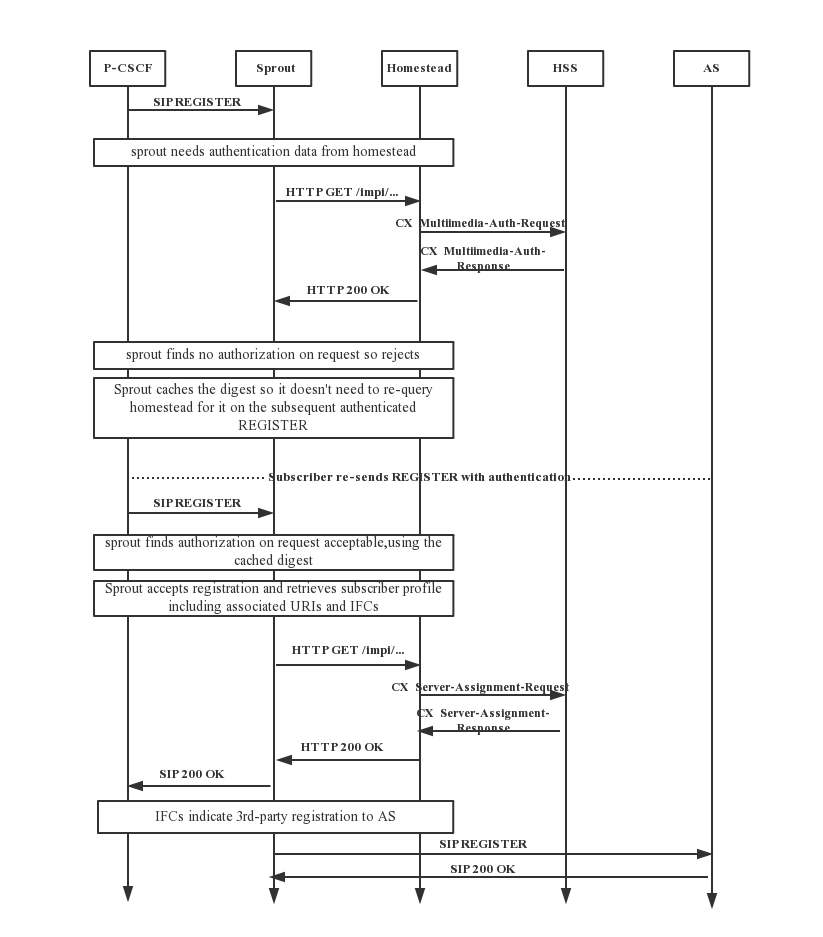
\includegraphics[width=1.0\textwidth]{clearwater/1.png}
	\bicaption[fig:flow_register]{用户注册服务流程图}{用户注册服务流程图}{Fig}{User Registration}
\end{figure}

\begin{figure}[!htp]
	\centering
	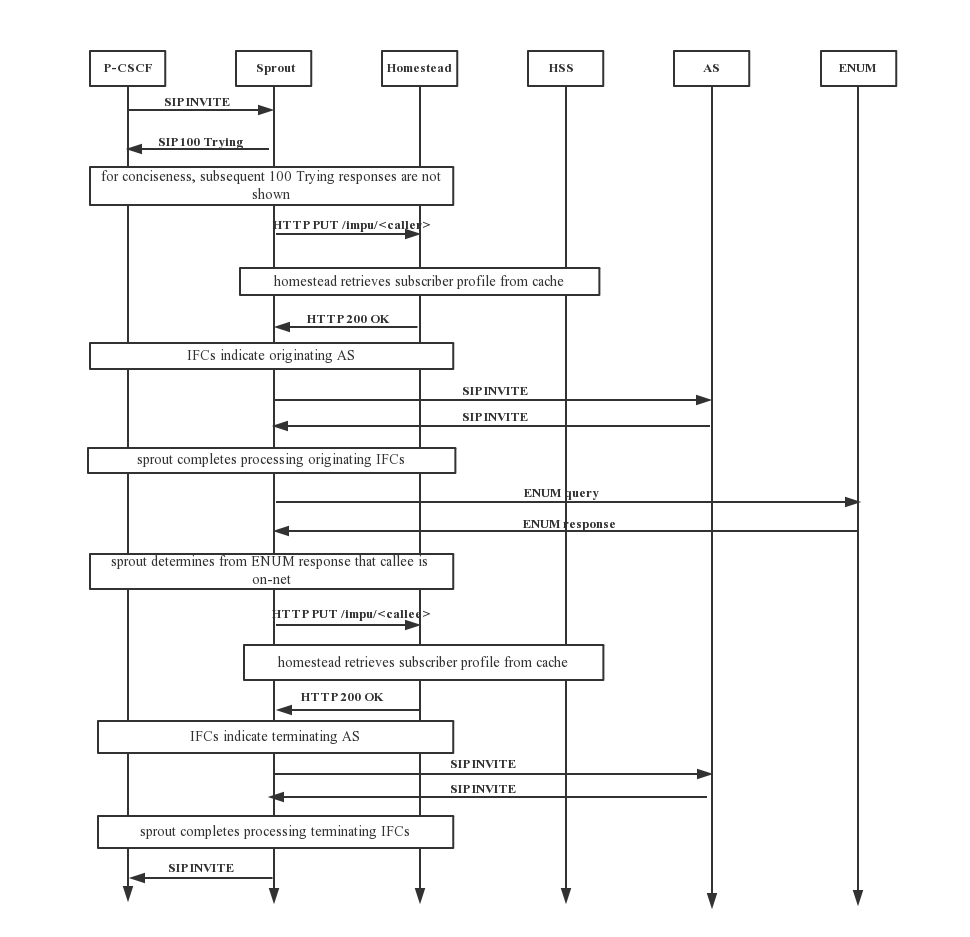
\includegraphics[width=1.0\textwidth]{clearwater/2.png}
	\bicaption[fig:flow_dialog]{初始化拨号流程}{初始化拨号流程}{Fig}{Init Dialog}
\end{figure}

\begin{figure}[!htp]
	\ContinuedFloat
	\centering
	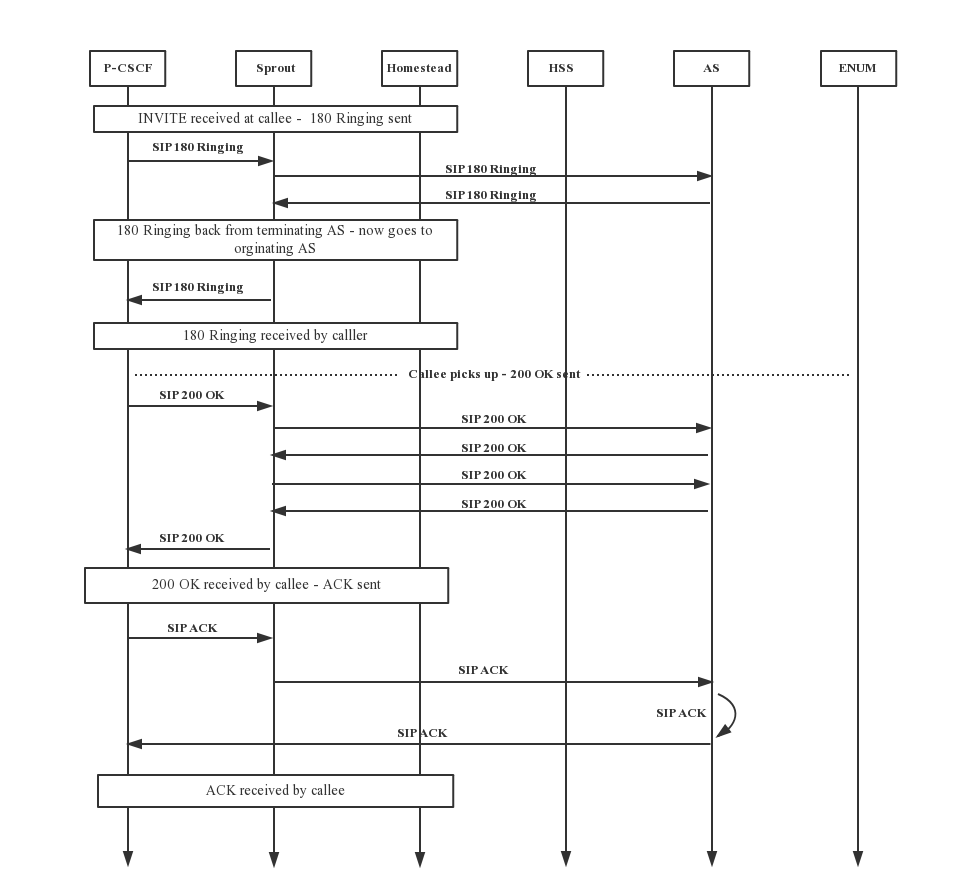
\includegraphics[width=1.0\textwidth]{clearwater/3.png}
	\bicaption[fig:flow_dialog2]{初始化拨号流程 (续)}{用户注册服务流程图}{Fig}{Init Dialog (con't)}
\end{figure}

\begin{figure}[!htp]
	\centering
	\label{fig:flow_inDialog}
	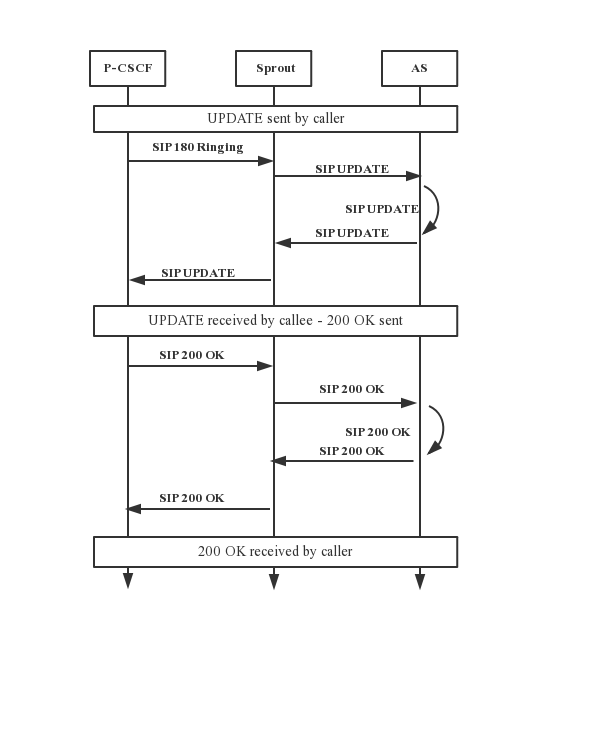
\includegraphics[width=1.0\textwidth]{clearwater/4.png}
	\bicaption[fig:flow_inDialog]{通话流程}{通话流程}{Fig}{In Dialog}
\end{figure}

\begin{figure}[!htp]
	\centering
	\label{fig:flow_terminate}
	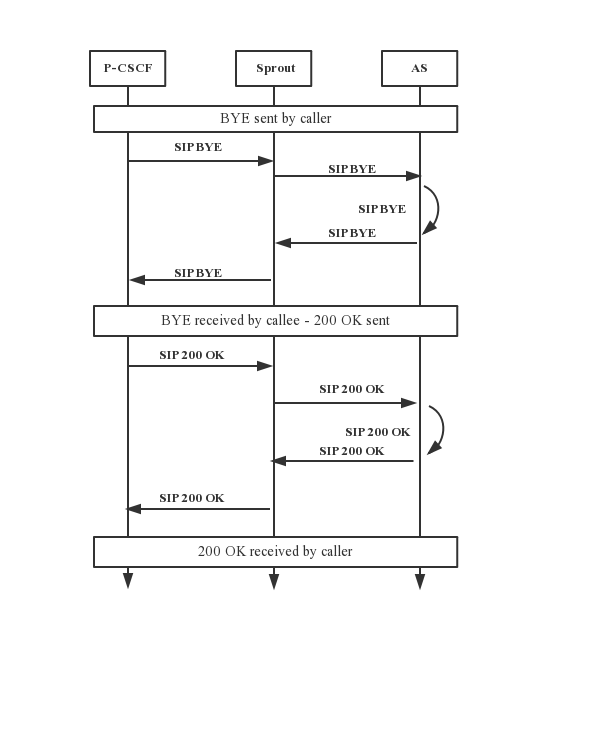
\includegraphics[width=1.0\textwidth]{clearwater/5.png}
	\bicaption[fig:flow_terminate]{通话终止流程}{通话终止流程}{Fig}{Terminate Dialog}
\end{figure}




\section{动态映射模块}
在该模块中,我们将需要根据服务链分析模块中生成的服务链组织链表通过算法 \ref{alg:greedy} 映射成为具体的实例链表,并根据实例链表完成服务链的组件。具体来说,我们在初始化阶段将所有的实例具体信息录入系统,包括其具体的网络功能、所分配的物理资源信息以及详细的配置参数。当具体的映射策略生成后,我们从实例列表中将实例的ip提出,通过绑定到DNS服务器的解析目录和转发列表中从而实现实例之间的物理链路组建。

\section{本章小结}
本章主要介绍了基于底层感知的高性能NFV平台的具体实现。详细介绍了平台的总体算法以及底层信息采样模块、服务链分析模块和动态映射模块的一些细节信息,给出了算法的伪代码实现以及实际服务链的流程分析。
\chapter{实验分析}
\label{chapter:evaluation}

\section{本章小结}
\chapter{全文总结}
\label{chapter:conclusion}

\section{主要结论}
网络功能虚拟化为传统电信业务描绘了十分美好的前景,是对已有电信架构的一次革新,大大提升了电信业务的开发效率,缩短了开发周期,降低了部署的成本。通过与现有的云计算基础设施相结合,网络功能虚拟化将实现服务的快速部署、伸缩和升级。然而,在从专有硬件向通用服务器迁移,软件化网络功能的过程中,不可避免地会遇到性能和服务质量下降的问题。特别是考虑到现有的大容量通用服务器中,多核的非一致性存储架构是被采用的主流架构,虚拟化的物力资源之间存在亲和度差异,不同亲和度的物理资源(CPU,内存等)之间的数据访问也会有较大的性能差异。这样的底层物理特性结合网络功能虚拟化中特殊的服务链结构,会引起很高的性能波动,导致服务质量下降。

本设计的研究内容主要着眼于通用的多核服务器中服务链的物理资源映射问题。在由成群的单核虚拟机所组成的服务节点集群,上层应用对特定服务的需求仅仅以服务链逻辑视图的方式体现,对于具体组成服务链的物理实例并不知晓,而在多核的非一致性存储访问平台下,被分配不同物理资源的虚拟机彼此之间具有一定的资源亲和度,即实例间的虚拟机访问性能与其物理资源的亲和度有较大的关系。这种底层资源的亲和度关系对于上层应用是透明的,也就是说上层服务在组织时并没有考虑到这层关系,所以可能会出现较大的性能波动。正是多核架构存在的这种亲和度关系,给我们组织服务链时,提供了新的解决思路。

基于以上的考虑,本设计中,我们对于多核物理核的非一致性存储访问和虚拟化相关技术进行了研究。当服务请求被发出时,通过解析请求,获取实际服务链的组成情况,结合底层资源亲和度的采样信息,采用基于贪心的搜索方法,构造理论上亲和度最好服务链映射关系,并同时考虑当前的运行负载,避免出现局部过热或资源竞争严重的不力情况。

最后,本文在实际的大容量通用服务器上,利用真实的网络服务Clearwater来验证了本设计的实现原型,并在真实的网络环境中对本设计进行了性能的评估。数据分析的结果表明,本设计在实验环境中可以平均可以减少40\%NFV具体业务服务延迟,并且在基础网络性能测试中,分别有最高30\%的延迟下降,300\%的带宽提升和20\%~\%60的吞吐提升。在使用相同数量的物理资源前提下,我们的设计显著地提高了资源的利用率。

\section{研究展望}
本设计虽然已经在通用的服务器上实现了初级原型并获得了一定了性能提升,但仍然存在一些可以提升和改进的空间。首先,本设计从单台服务器的物理资源亲和度角度出发,而在实际生产环境中,尤其是云计算数据中心中,机架上的服务器都是以高性能网卡相连所组成的服务器集群,我们的资源亲和度模型可以扩展到多台物理机的范围。另外本文所提出的映射算法在问题规模较小的前提下具有很好的效果,但是当问题规模扩展到一定级别,算法的执行效率会大大下降,这时候需要结合一些已有的高级算法来提升算法的时间消耗以满足实际生产中的响应需求。

希望本文所完成的工作能够具有一些抛砖引玉的积极作用,为其他研究者在网络功能虚拟化及虚拟机调度方向的研究提供有益的帮助和参考。

%\include{tex/intro}
%\include{tex/example}
%\include{tex/faq}
%\include{tex/summary}

\appendix	% 使用英文字母对附录编号,重新定义附录中的公式、图图表编号样式
\renewcommand\theequation{\Alph{chapter}--\arabic{equation}}	
\renewcommand\thefigure{\Alph{chapter}--\arabic{figure}}
\renewcommand\thetable{\Alph{chapter}--\arabic{table}}
\renewcommand\thealgorithm{\Alph{chapter}--\arabic{algorithm}}

%% 附录内容,本科学位论文可以用翻译的文献替代。
%\include{tex/app_setup}
%\include{tex/app_eq}
%\include{tex/app_cjk}
%\include{tex/app_log}

\backmatter	% 文后无编号部分 

%% 参考资料
\printbibliography[heading=bibintoc]

%% 致谢、发表论文、申请专利、参与项目、简历
%% 用于盲审的论文需隐去致谢、发表论文、申请专利、参与的项目
\makeatletter

%%
% "研究生学位论文送盲审印刷格式的统一要求"
% http://www.gs.sjtu.edu.cn/inform/3/2015/20151120_123928_738.htm

% 盲审删去删去致谢页
\ifsjtu@review\relax\else
  %# -*- coding: utf-8-unix -*-
\begin{thanks}
我首先要感谢的是我的导师李健副教授。在科研上,李老师对我的教导和支持具有重要意义,我的科研成果离不开李老师的指导。在本人的研究生阶段的学习和生活中,李老师严谨治学的态度、开阔的视野和灵活的思维给我留下了深刻的印象。李老师不厌其烦地帮助我整理思路,解决科研上遇到的各种困难,尤其是撰写论文方面,提出了许多关键性的意见和建议,对我的帮助非常大。在研究生期间,我的课题研究能够顺利完成,离不开李老师的悉心指导。借此机会谨向李老师表达诚挚的敬意和真诚的感谢。

特别感谢我的另一位指导老师马汝辉老师,马老师科研经验丰富,思维敏捷,视野开阔。当我在科研上遇到的阻力时,马老师会耐心地给我指明方向,鼓励我坚持不懈攻克难关。	

非常感谢实验室中与我一起的所有的同学,他们帮助我客服生活和科研上的种种困难,陪我度过了人生中充满意义的研究生时光。感谢实验室的两位博士钱建民和胡小康,他们无私地分享自己的研究经验,在科研上技术上给了我许多重要的支持。与同学们一起学习、一起研究的岁月我必将一生难忘。

最后,特别感谢我的父母和我的家人,是我父母的培养给我了接受研究生教育的机会,我的所有进步和所取得的所有成绩都离不开你们的理解、支持和鼓励,你们永远是我最坚实的后盾。


\end{thanks}
 	  %% 致谢
\fi

\ifsjtu@bachelor
  % 学士学位论文要求在最后有一个英文大摘要,单独编页码
  \pagestyle{biglast}
  \include{tex/end_english_abstract}
\else
  % 盲审论文中,发表学术论文及参与科研情况等仅以第几作者注明即可,不要出现作者或他人姓名
  \ifsjtu@review\relax
    %# -*- coding: utf-8-unix -*-

\begin{publications}{99}
    \item\textsc{第一作者}. {EI国际会议论文}, 2017.
\end{publications}

    \include{tex/projectsreview}  
  \else
    %# -*- coding: utf-8-unix -*-
%%==================================================
%% pub.tex for SJTUThesis
%% Encoding: UTF-8
%%==================================================

\begin{publications}{99}
    \item\textsc{Yangde Li, Hao Yin}. {Data Path Profiling for Network Function Virtualization }[C]. International Conference on Computer and Communications , 2017.
\end{publications}
	      %% 发表论文
    \include{tex/projects}  %% 参与的项目
  \fi
\fi

% %# -*- coding: utf-8-unix -*-
\begin{patents}{99}
    \item 第二发明人,“虚拟化多核环境下非一致性I/O访问虚拟机资源迁移方法”,专利申请号201610415935.5
    \item 第二发明人,“一种基于底层NUMA感知的NFV实现方法”,专利申请号291710209194.X
\end{patents}
	  %% 申请专利
% \include{tex/resume}	  %% 个人简历

\makeatother

\end{document}
